\section{Event Topology and Spherical Harmonics Analysis}
\label{sec:topology_and_harmonics}

In this section we provide details about spherical harmonics analysis to separate 0\nbb-decay signal events from backgrounds. 
We show that spherical harmonics decomposition of the PE hits on the detector surface is sensitive to the event topology. In particular
we focus on the differences between two-electron (0\nbb-decay events) and single-electron (\B~events) topologies. More complicated 
event topologies such as \C~background events are also differ from two-electron signal topology. However, as explained further in 
Sec.~\ref{subsec:c10_spherical_harmonics}, the 0\nbb/\C~separation power strongly depends on the assumptions that are built into the 
simulation. Therefore we use only 0\nbb/\B~separation as a benchmark test for the spherical harmonics analysis performance.


\subsection{Topology of 0\nbb-decay and \B~Events}
\label{subsec:topology}

When a typical 0\nbb-decay candidate isotope is considered, all \B~background events will have that single electron above Cherenkov threshold
in a liquid scintillator. Also a large fraction of 0\nbb-decay signal events will have both electrons above Cherenkov threshold. Cherenkov photons
from each of the electrons will produce ring shaped clusters of PE hits on the detecor surface. Therefore, any event reconstruction algorithm 
that is capable of separating events with one Cherenkov cluster from events with two Cherenkov clusters should have signal-background 
descrimination power. 

In some cases only one Cherenkov cluster is produced in 0\nbb-decay signal events. This happens either when the angle between the two 
0\nbb-decay electrons is small and Cherenkov clusters overlap or when the energy split between electrons is not balanced causing 
one electron to be below Cherenkov threshold.
Such signal events cannot be separated from background based on topology of the Cherenkov photons distribution on the detector surface. 
However directionality of the electron that is above Cherenkov threshold can still be resonctructed. This directionality information would allow
for \B~events suppresion based on the position of the sun.

Identification of the Cherenkov clusters is challenging due to much higher amount of uniformly distributed scintillation ligth that is
produced in every event. We found that spherical harmonics analysis on an early PE sample which has relatively high fraction of 
Cherenkov PE makes it possile to separate some of the 0\nbb-decay signal events from backgrounds.

\subsection{Description of Spherical Harmonics Analysis}

For the purpose of illustration of the spherical harmonics analysis concept we first consider three distinct topologies: 
two electrons produced back-to-back at an 180$^{\circ}$ angle, two electrons at a 90$^{\circ}$ angle, and a single electron.
Figure~\ref{fig:ThreeTopologies_Display_5MeV} shows an idealized simulation of these three topologies for the total electrons 
energy of 10~MeV. In order to emphasize ring patterns formed by cherenkov photons the electron multiple scattering process is turned off
in this idealized simulation. Here the single-electron event represents an idealized \B~event topology and the two-electron events represent
two special cases of an idealized 0\nbb-decay topology.


\begin{figure*}[h]
  \centering
%  \begin{tabular}{c c c}
  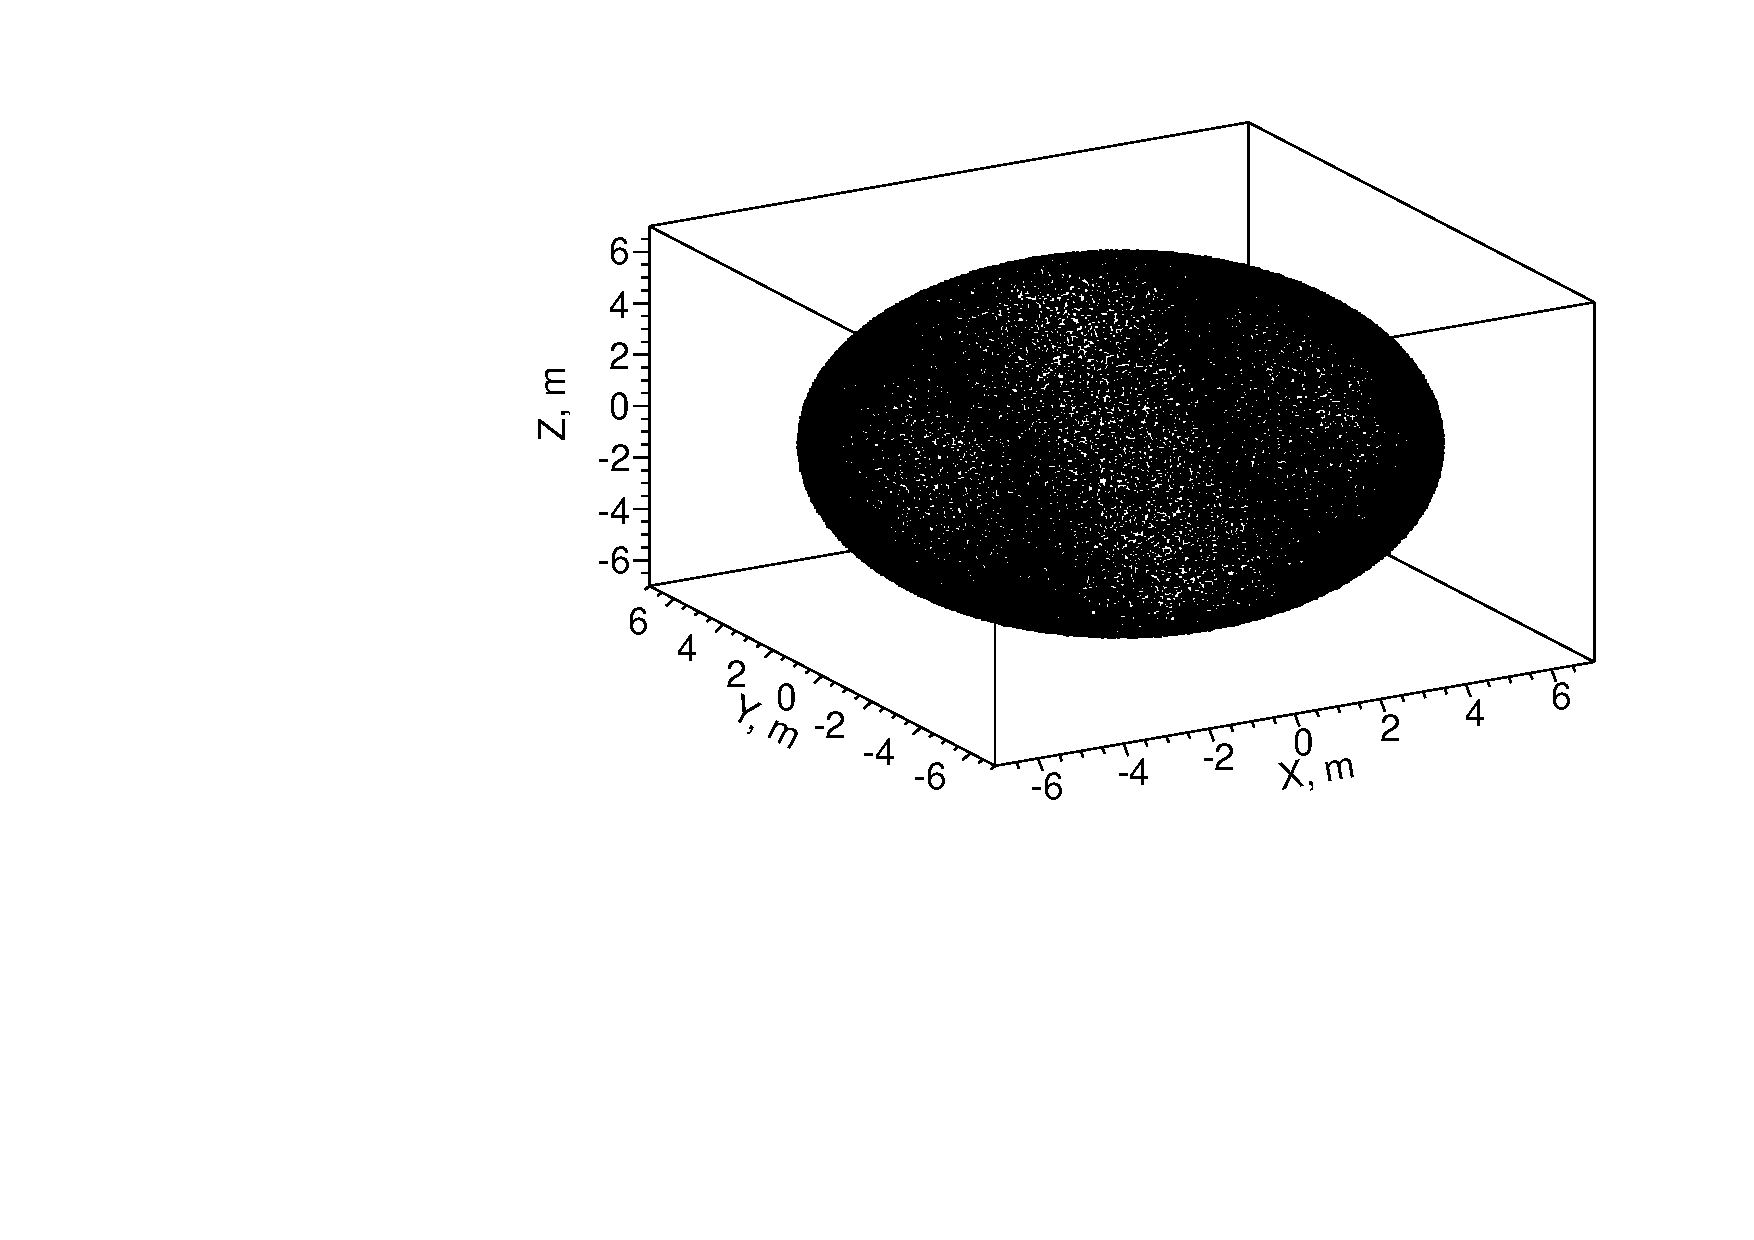
\includegraphics[width=0.45\textwidth]{hDisplay_topology180_5MeV.pdf}
  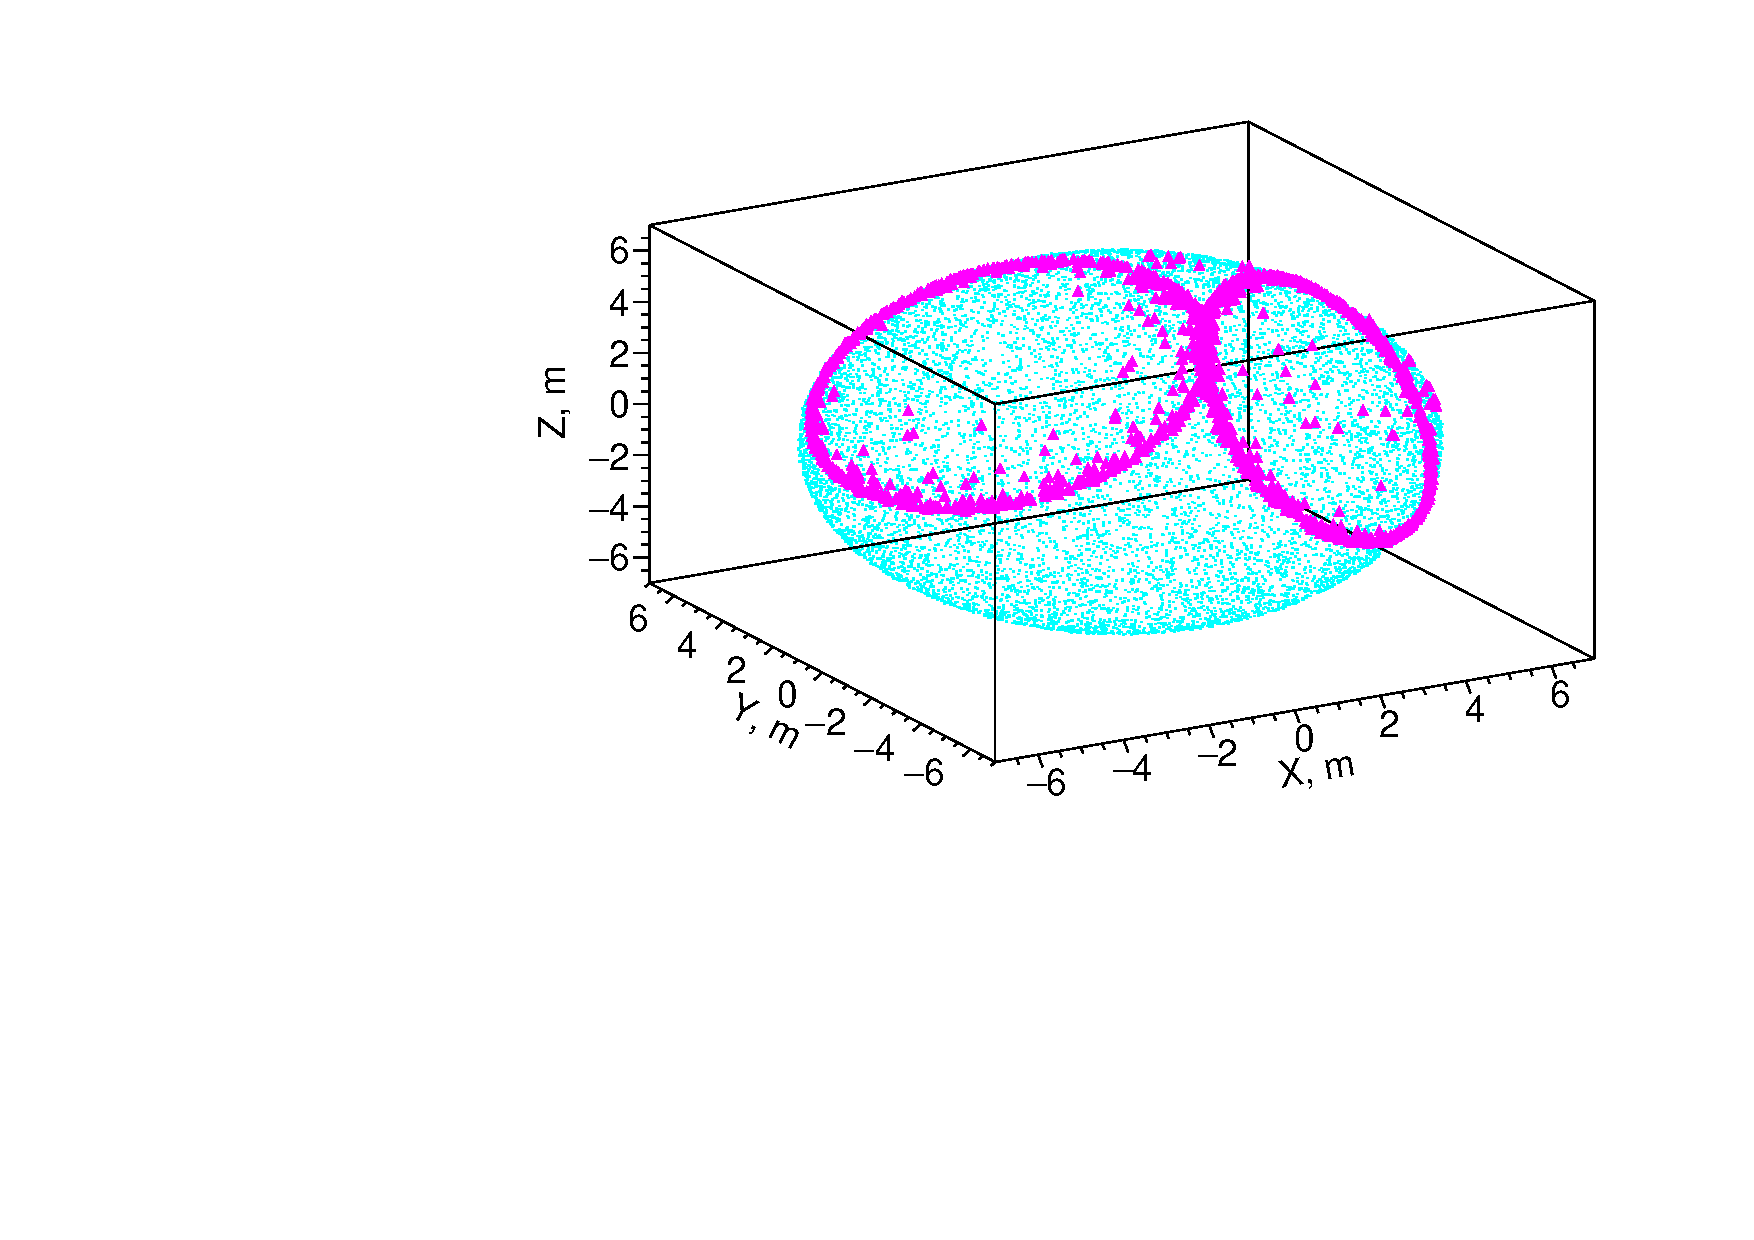
\includegraphics[width=0.45\textwidth]{hDisplay_topology90_5MeV.pdf}
  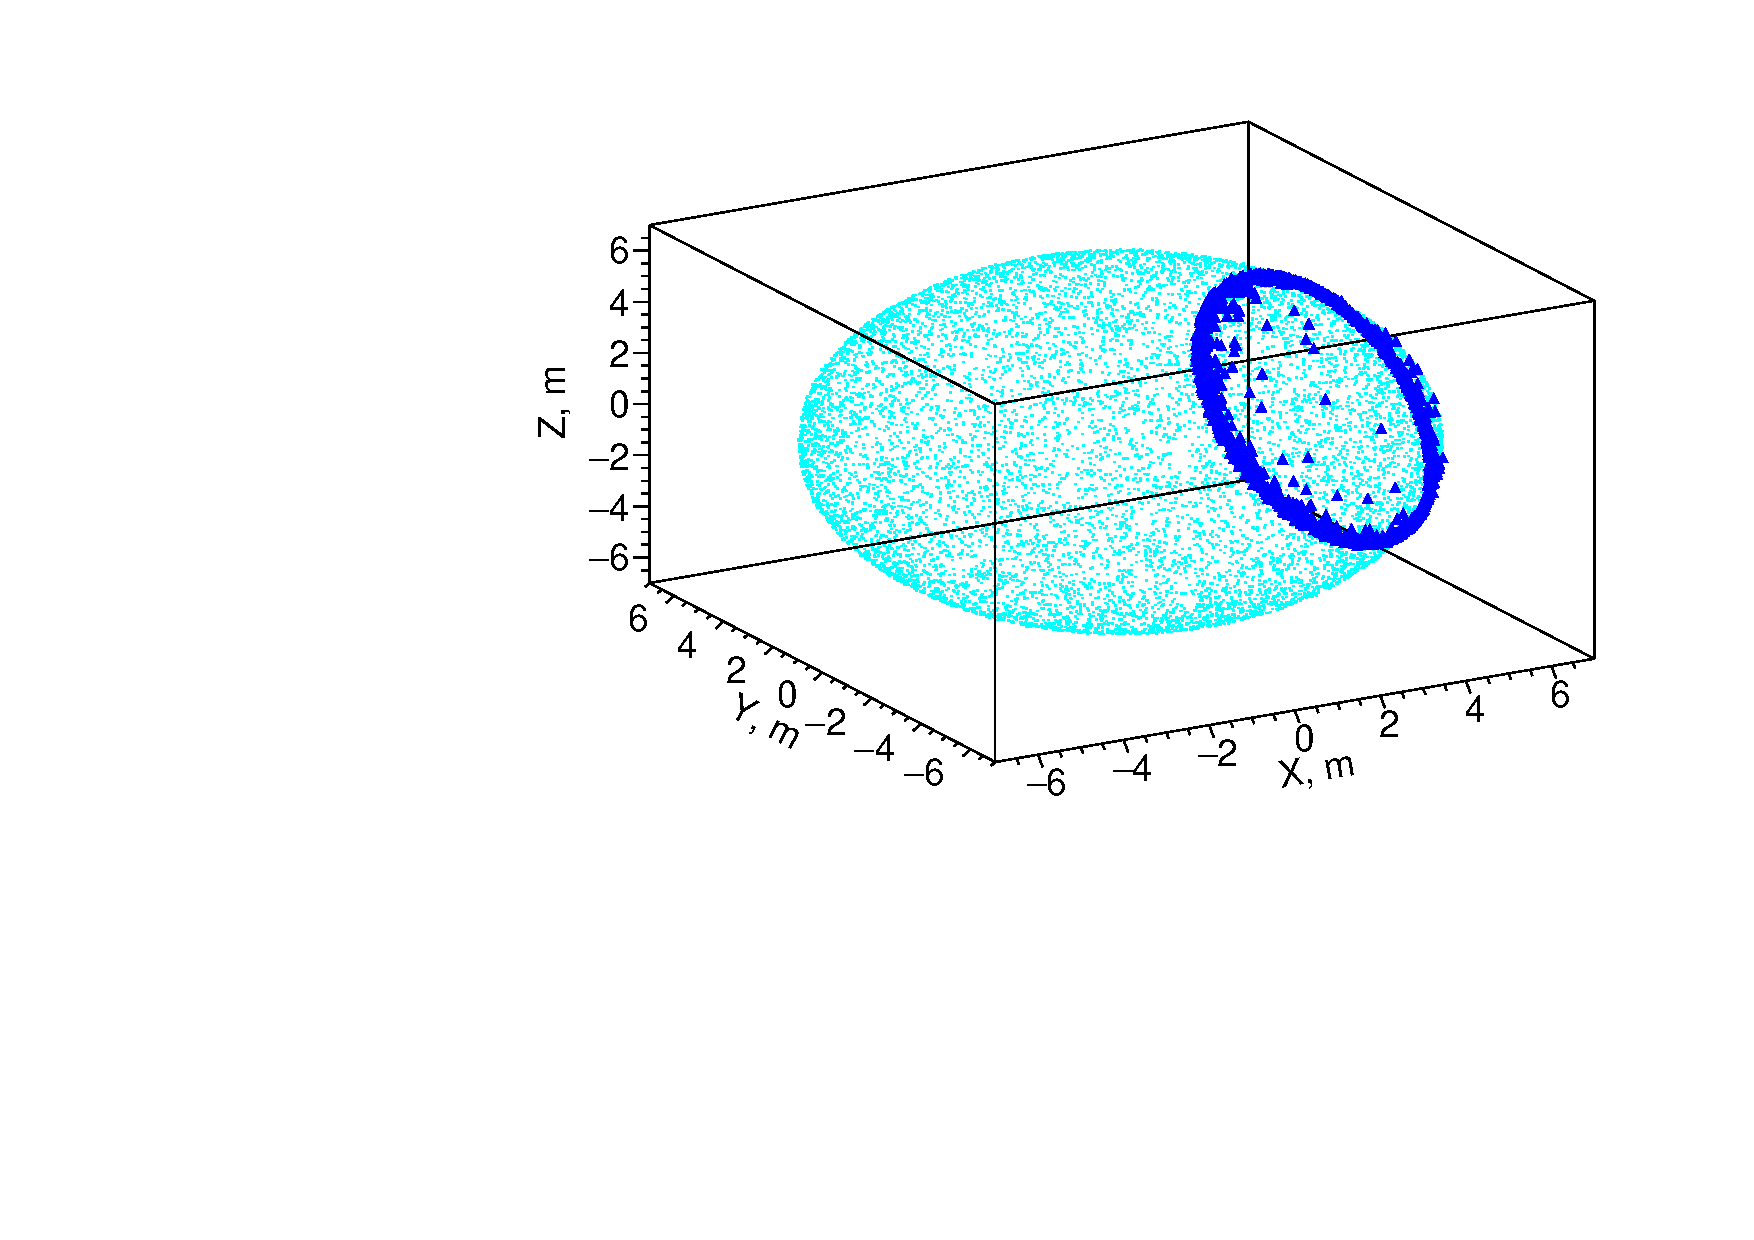
\includegraphics[width=0.45\textwidth]{hDisplay_1el_10MeV.pdf}
%  \end{tabular}
  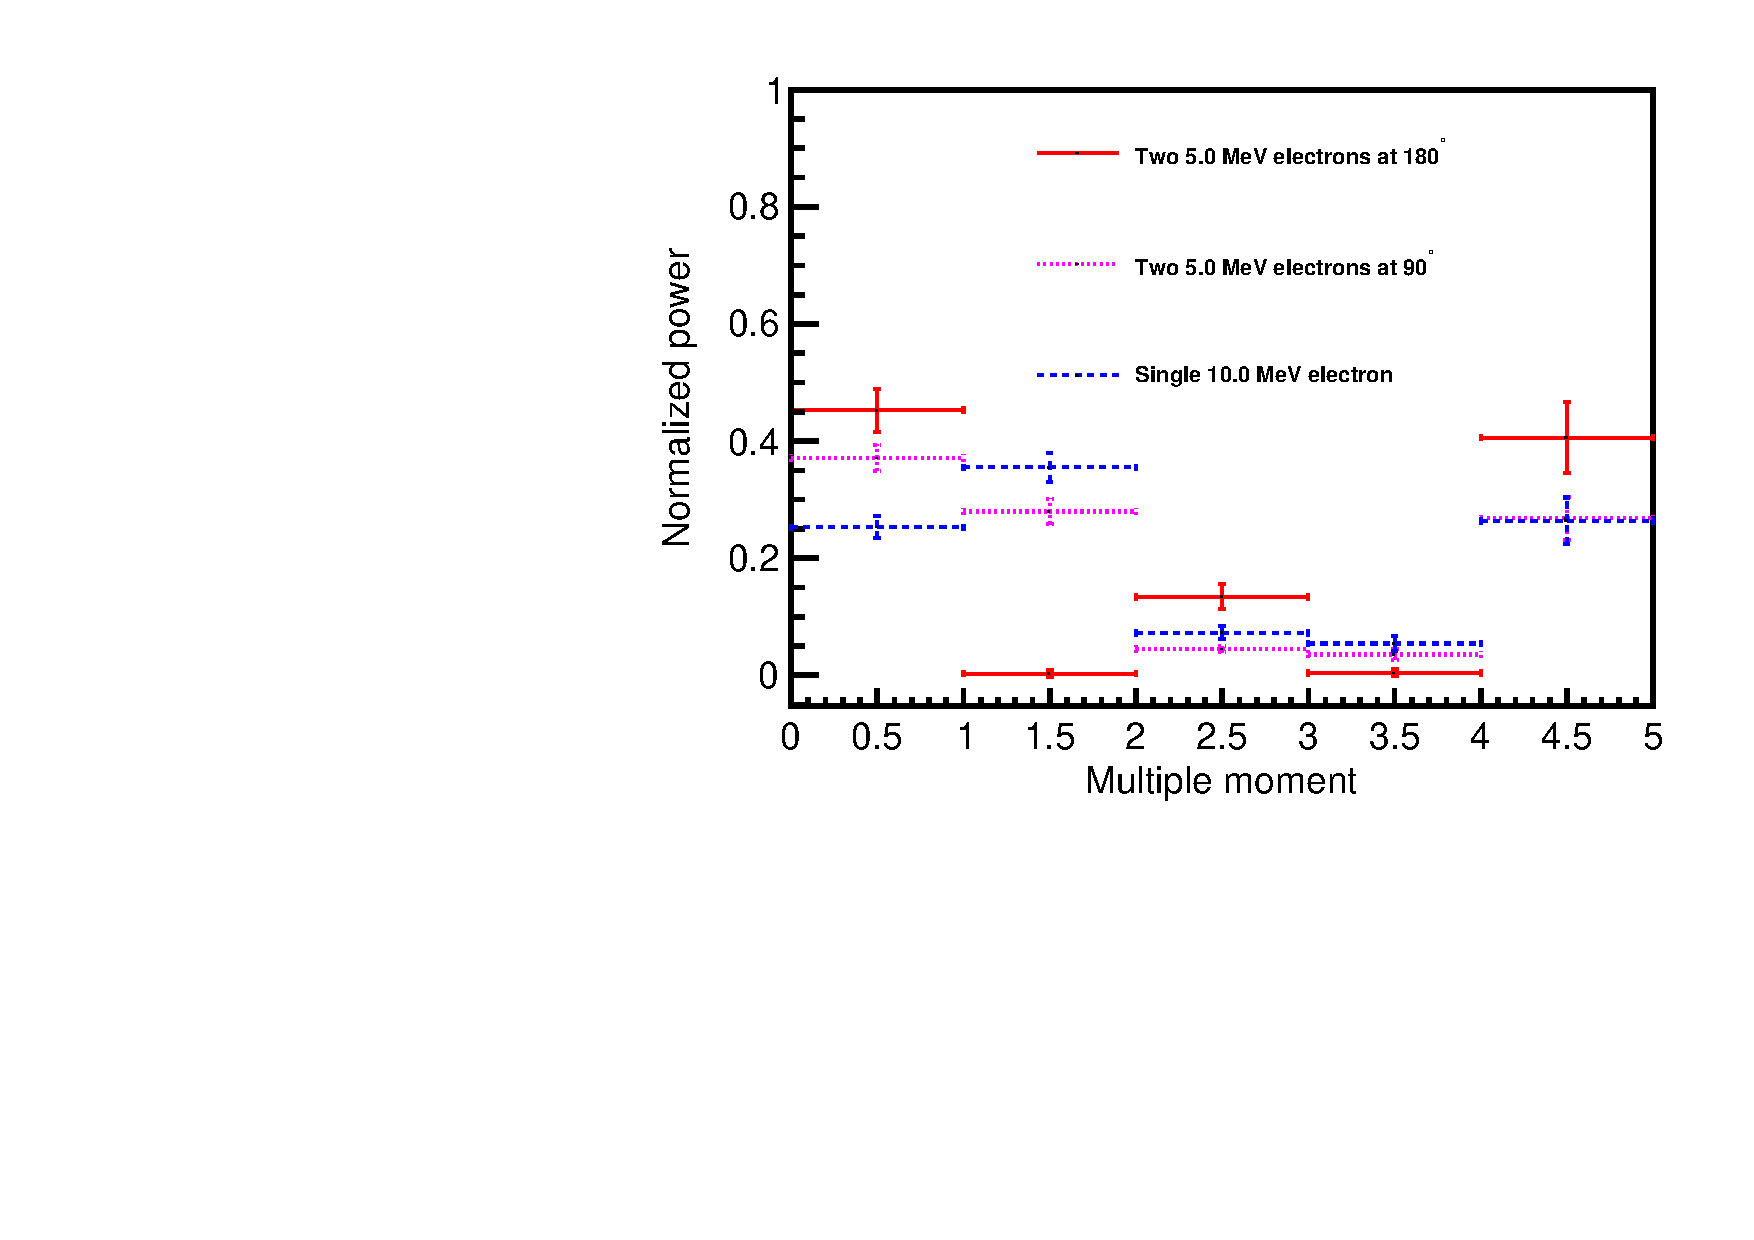
\includegraphics[width=0.45\textwidth]{hMultipleMoment_CHELight_VtxSmear0cm_VtxShiftX0cm_999p9ns_5p0MeV_center_NoMultScat.pdf}
  \caption{\emph{Top pannels and bottom left pannel:} Idealized event displays for the three representative event topologies: two 5~MeV 
    back-to-back electrons (\emph{top left}), two 5~MeV electrons at 90$^{\circ}$ angle (\emph{top right}), and a single 10~MeV electron
    (\emph{bottom right}). Multiple scattering is turned off in the simulation to emphasize the difference in the mutual orientation of
    cherenkov rings for the three topologies. For the illustration purposes 100\% QE is applied to cherenkov photons (triangles)
    and the default QE is applied to scintillation photons (dots). All electrons originate at the center of the
    detector. One typical event is shown for each topology.
    \emph{Bottom right pannel:} Normalized power spectrum $S_l$ calculated for distribution of cherenkov photons only. The three
    topologies are compared: two 5~MeV back-to-back electrons (\emph{solid red line}), two 5~MeV electrons at 90$^{\circ}$ angle
    (\emph{dotted magenta line}), and a single 10~MeV electron (\emph{dashed blue line}). For each topology 100 events were simulated. 
    The normalized power values $S_l$'s were calculated for each individual event. The horizontal lines correspond to the mean values of 
    $S_l$ within each event topology. The vertical bars show one standard deviation from the mean value.}
  \label{fig:ThreeTopologies_Display_5MeV}
\end{figure*}



The central strategy of the spherical harmonics analysis is to construct rotationally invariant variables that can be used to separate 
different event topologies. To this end, let the  function $f(\theta,\phi)$ represent the PE distribution on the detector surface. The function $f(\theta,\phi)$ can be decomposed into a sum of spherical harmonics:

\begin{eqnarray}
\label{eq1}
f(\theta,\phi) = \sum_{l=0}^{\infty} \sum_{m=-l}^{l} f_{lm} Y_{lm}(\theta,\phi),
\end{eqnarray}

where $Y_{lm}$ are Laplace's spherical harmonics defined in a real-value basis using Legendre polynomials $P_l$:

\begin{eqnarray}
\label{eq2}
Y_{lm} = \left\{
  \begin{array}{@{}ll@{}}
    \sqrt{2}N_{lm}P_l^m(cos\theta)cos~m\phi, & \text{if}\ m>0 \\
    N_{lm} = \sqrt{\frac{(2l+1)}{4\pi} \frac{(l-m)!}{(l+m)!}}, & \text{if}\ m=0 \\
    \sqrt{2}N_{l|m|}P_l^{|m|}(cos\theta)sin~|m|\phi, & \text{if}\ m<0
  \end{array}\right.
\end{eqnarray}

where the coefficients $f_{lm}$ are defined as
 
\begin{eqnarray}
\label{eq3}
f_{lm} = \int_{0}^{2\pi} d\phi \int_0^{\pi} d\theta sin\theta f(\theta,\phi) Y_{lm}(\theta,\phi).
\end{eqnarray}

Equation~\ref{eq4} defines the power spectrum of $f(\theta,\phi)$ in the spherical harmonics representation, $s_l$, where $l$ is a multiple moment. The power spectrum, $s_l$, is invariant under rotation. It is unique to each of the functions $f_i(\theta,\phi)$, $i=$1,2,3..., which can not be transformed into each other by rotation.

\begin{eqnarray}
\label{eq4}
s_l = \sum_{m=-l}^{m=l} |f_{lm}|^2
\end{eqnarray}

The event topology in a spherical detector determines the distribution of the PE's on the detector sphere, and, therefore, a set of $s_l$'s. These values can serve as a quantitative figure of merit for different event topologies. The rotation invariance of $s_l$'s ensures that this figure of merit does not depend on the orientation of the event with respect to the chosen coordinate frame.

Sum of $s_l$'s over all multiple moments equals to the L2 norm of the function $f(\theta,\phi)$:

\begin{eqnarray}
\label{eq5}
\sum_{l=0}^{\infty} s_l = \int_{\Omega} |f(\theta,\phi)|^2 d\Omega.
\end{eqnarray}

Therefore, the normalized power spectrum,

\begin{eqnarray}
\label{eq6}
S_l = \frac{s_l}{\sum_{l=0}^{\infty} s_l} =  \frac{s_l}{\int_{\Omega} |f(\theta,\phi)|^2 d\Omega},
\end{eqnarray}

can be used to compare shapes of various functions $f(\theta,\phi)$ with different normalization. The total number of PEs detected on the detector sphere fluctuates from event to event, therefore, in all of the following we use the normalized power $S_l$.

Figure~\ref{fig:ThreeTopologies_Display_5MeV}(\emph(bottom right)) compares the normalized power spectra for the three representative event topologies.
There is sufficien separation between these three idealized event topologies.

In practice, at energies relevant to 0\nbb-decay Cherenkov rings become very fuzzy due to elecron multiple scattering. In most cases $\sim$1~MeV 
electrons produce randomly shaped clusters of Cherenkov photons around the direction of the electron track. Examples of such Cherenkov clusters
for the same three representative topologies are shown in Fig.~\ref{fig:ThreeTopologies_Display}. Now the multiple scattering process is included 
in the simulation and the total kinetic energy of the electrons is equal to the Q-value of the \Te.


\begin{figure*}[h]
  \centering
%  \begin{tabular}{c c c}
  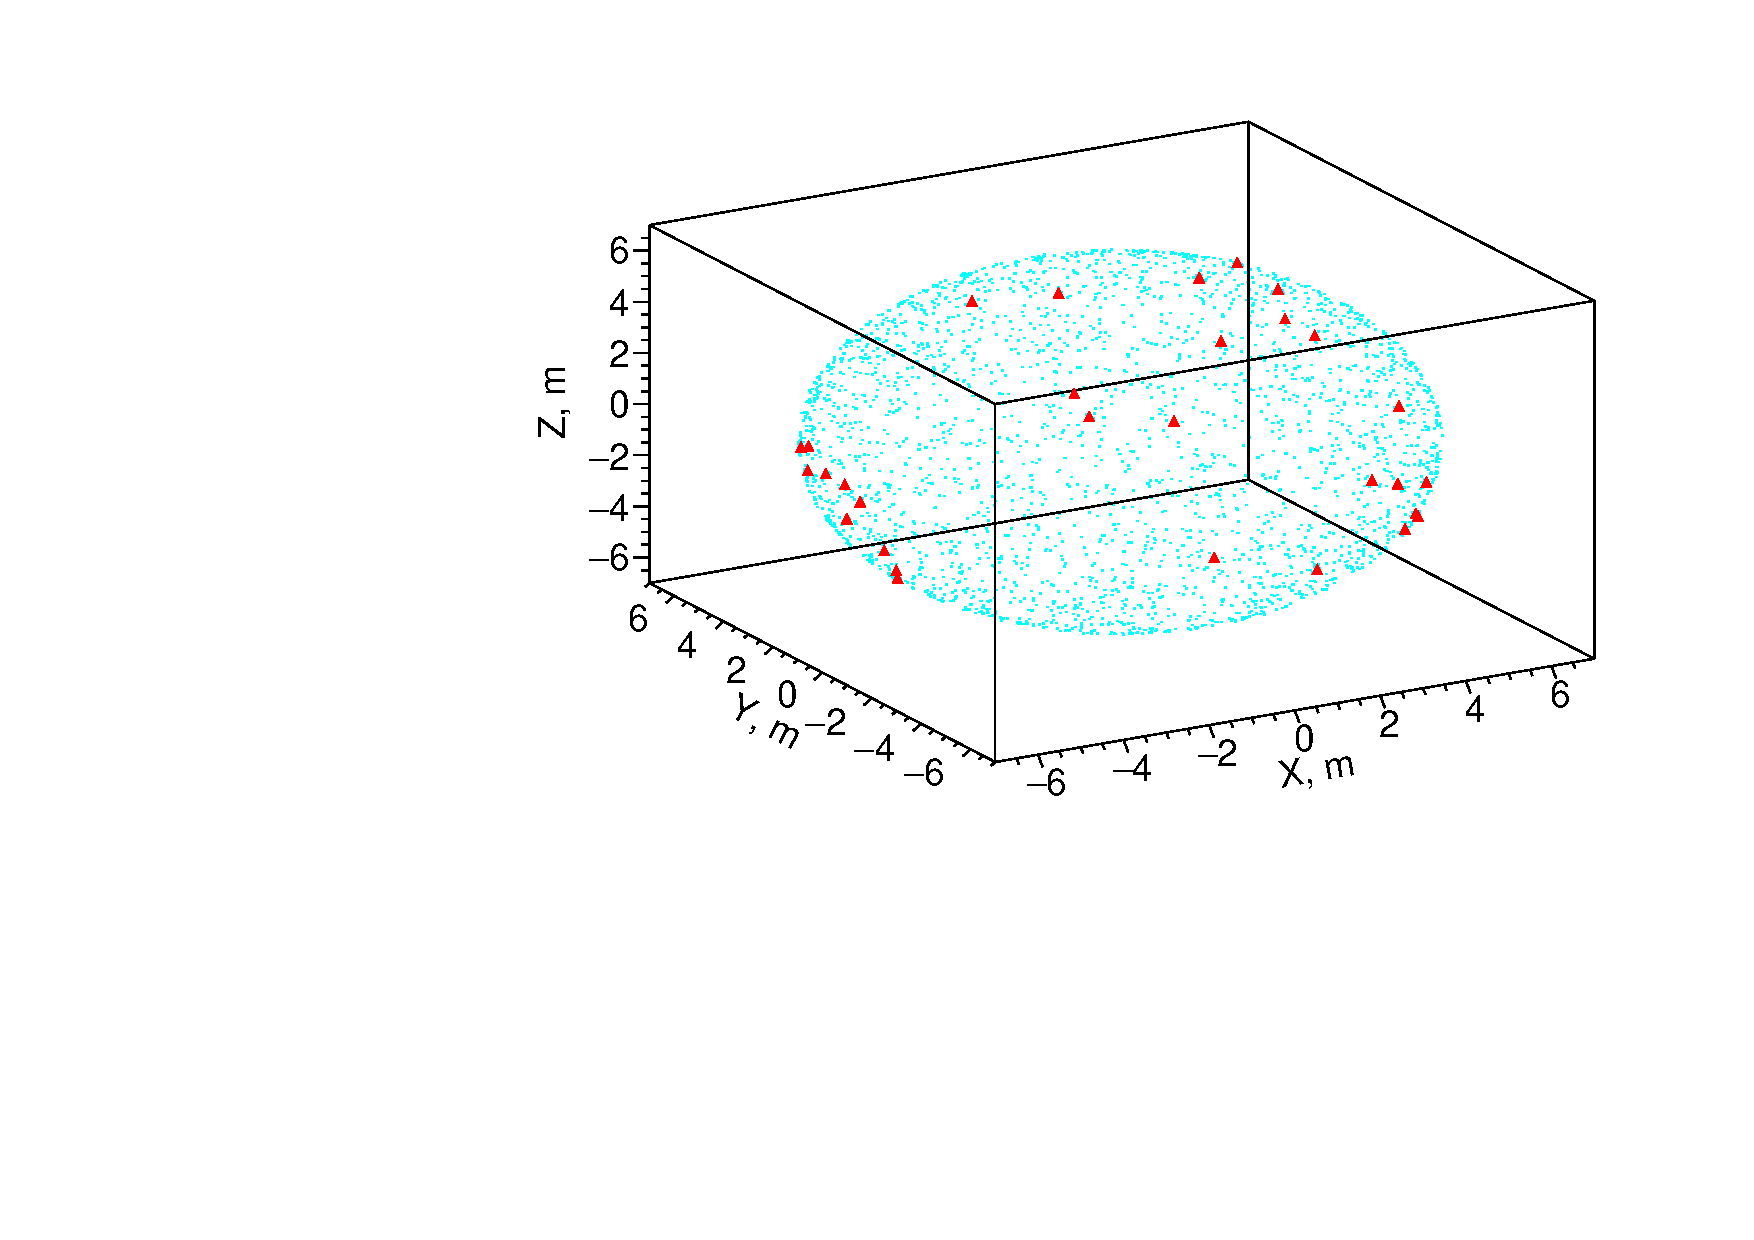
\includegraphics[width=0.45\textwidth]{hDisplay_topology180_2p529MeVTot}
  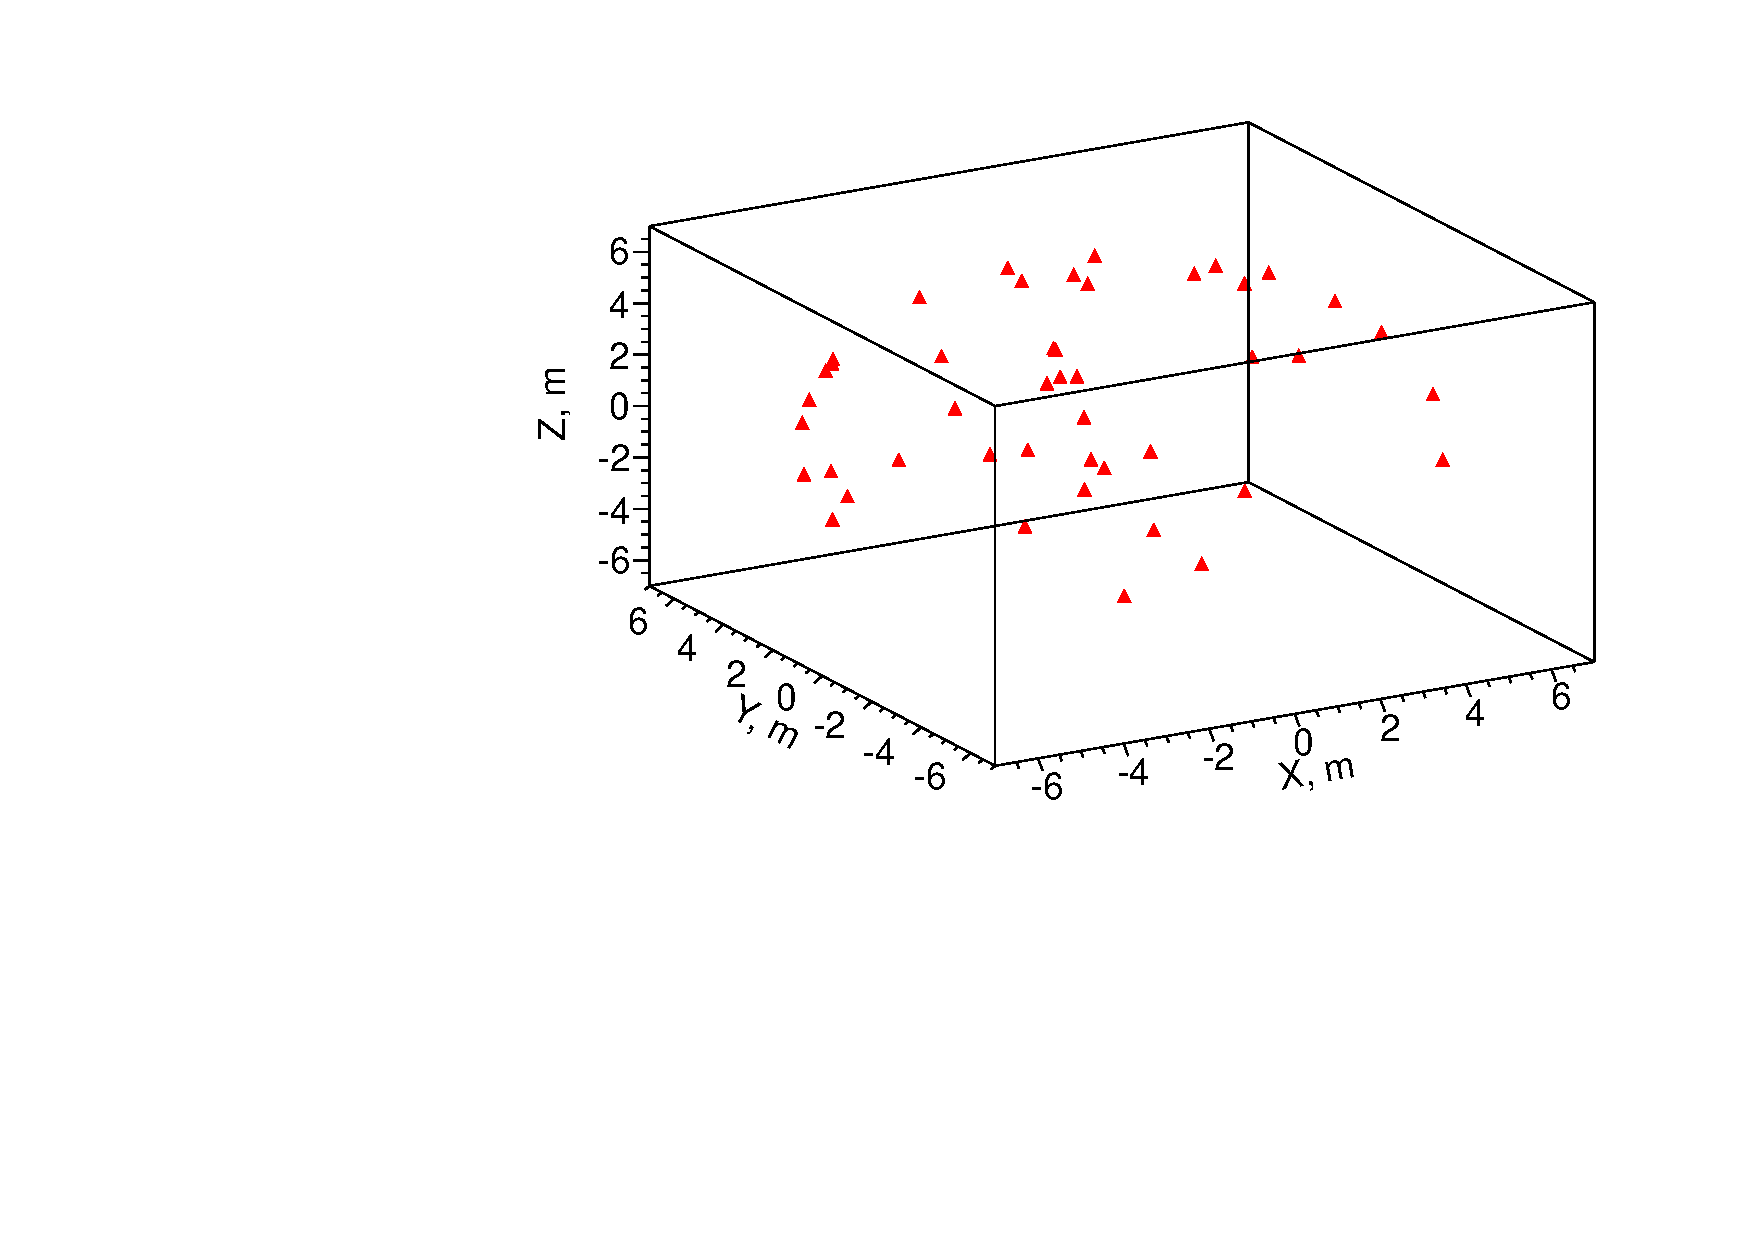
\includegraphics[width=0.45\textwidth]{hDisplay_topology90_2p529MeVTot}
  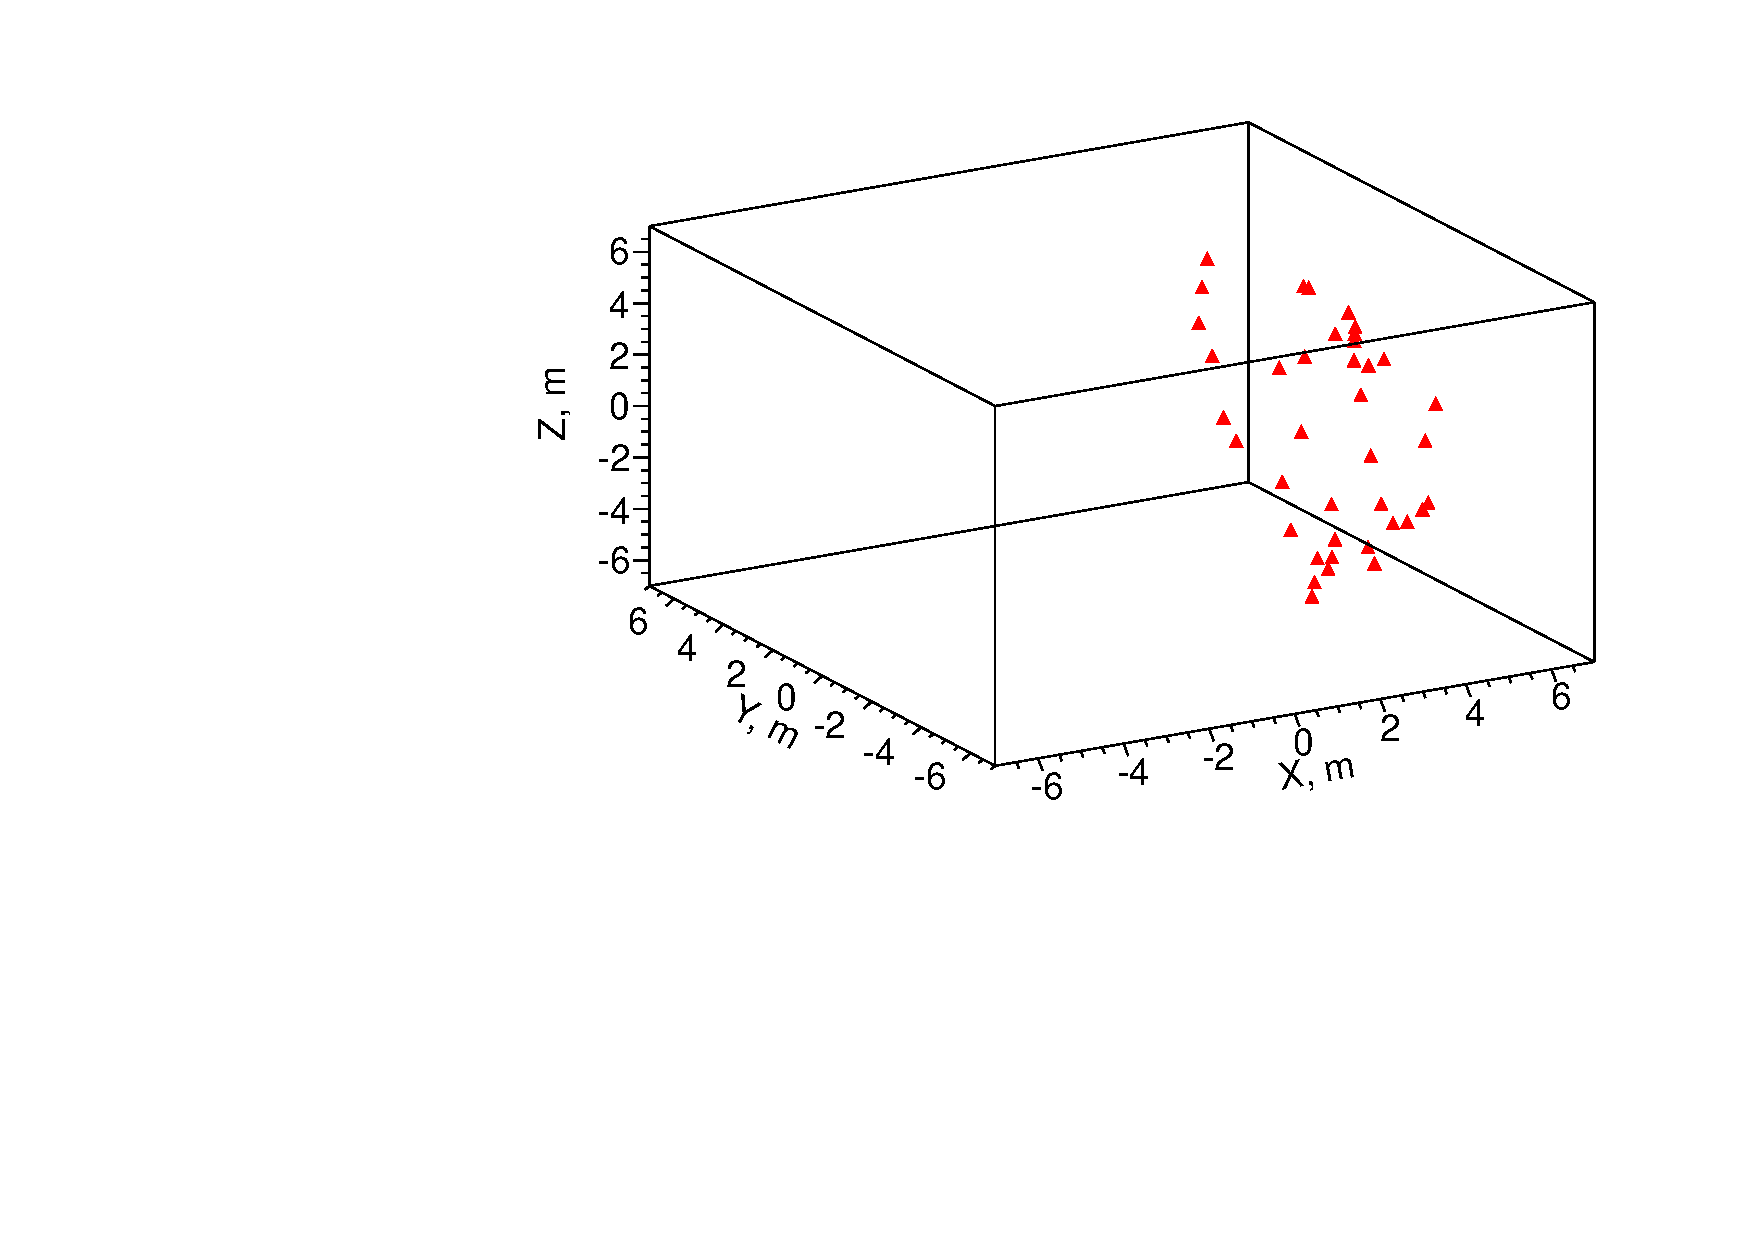
\includegraphics[width=0.45\textwidth]{hDisplay_1el_2p529MeV}
%  \end{tabular}
  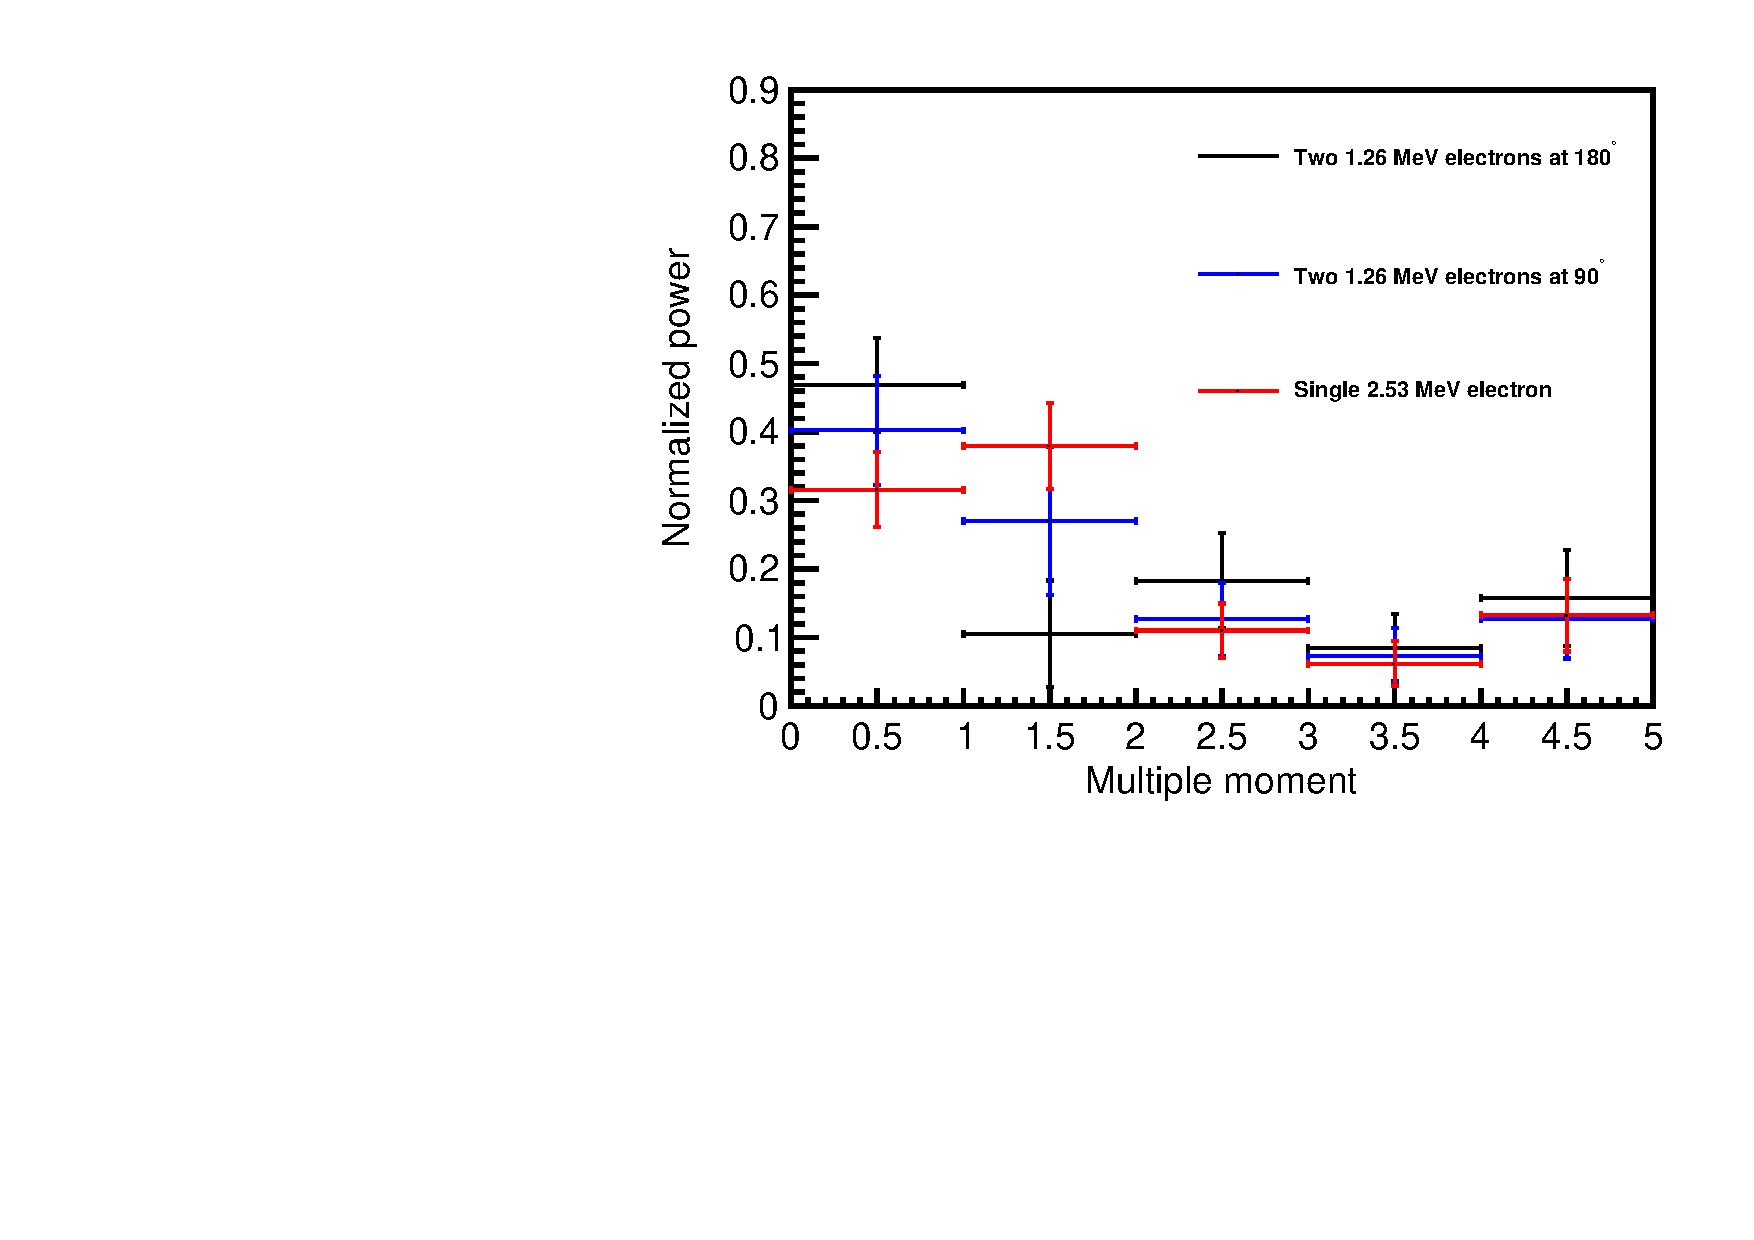
\includegraphics[width=0.45\textwidth]{hMultipleMoment_cheLight_VtxSmear0cm_VtxShiftX0cm_999p9ns_center.pdf}
  \caption{\emph{Top pannels and bottom left pannel:} Event displays for the three representative event topologies with the electron energies relevant 
    for the {\Te} 0{\nbb}-decay: two back-to-back 1.26~MeV electrons (\emph{top left}), two 1.26~MeV electrons at 90$^{\circ}$ angle 
    (\emph{top right}), and a single 2.53~MeV electron (\emph{bottom left}). Multiple scattering is now properly included in the simulation
    For the illustration purposes 100\% QE is applied to cherenkov photons (triangles) and the default QE is applied to scintillation 
    photons (dots). All electrons originate at the center of the detector. One typical event is shown for each topology.
    \emph{Bottom right pannel:} Normalized power spectrum $S_l$ calculated for distribution of cherenkov photons only. The three
    topologies are compared: two back-to-back 1.26~MeV electrons (\emph{solid red line}), two 1.26~MeV electrons at 90$^{\circ}$ angle
    (\emph{dotted magenta line}), and a single 2.53~MeV electron (\emph{dashed blue line}). For each topology 1000 events were simulated.
    The normalized power values $S_l$'s were calculated for each individual event. The horizontal lines correspond to the mean values of
    $S_l$ within each event topology. The vertical bars show one standard deviation from the mean value.}
  \label{fig:ThreeTopologies_Display}
\end{figure*}


At 2.53~MeV with multiple scattering included the difference in the Cherenkov photon distribution for the three representative topologies 
is not as dramatic as in the idealized simulation of 10~MeV events. However, a guess about the event topology still can be made by comparing 
photon distributions in different segments of the detector sphere. Spherical harmonics decomposotion is a natural tool for making such 
comparison between the segments. As shown in Fig.~\ref{fig:ThreeTopologies_Display}~(\emph{bottom right}) spherical harmonics power spectrum 
of Cherenkov photons only still provides noticable separation between all three event topologies.

More realistic examples of \Te~ 0\nbb~and \B~events simulated at the center of the detector are shown in Fig.~\ref{fig:Te130_Display}. 
Early photoelectrons (PEs), defined as those PEs from Cherenkov and scintillation light within 33.5~ns of the start of the event, are shown. 
The default QE is applied.  In this more realistic example, the uniformly distributed scintillation light makes it more difficult to 
visually distinguish the event topology. Nevertheless, Fig.~\ref{fig:Te130_Display}~(\emph{bottom panne}) shows that the spherical harmonics
analysis still finds differences between two-track and single-track events.

\begin{figure*}[h]
  \centering
  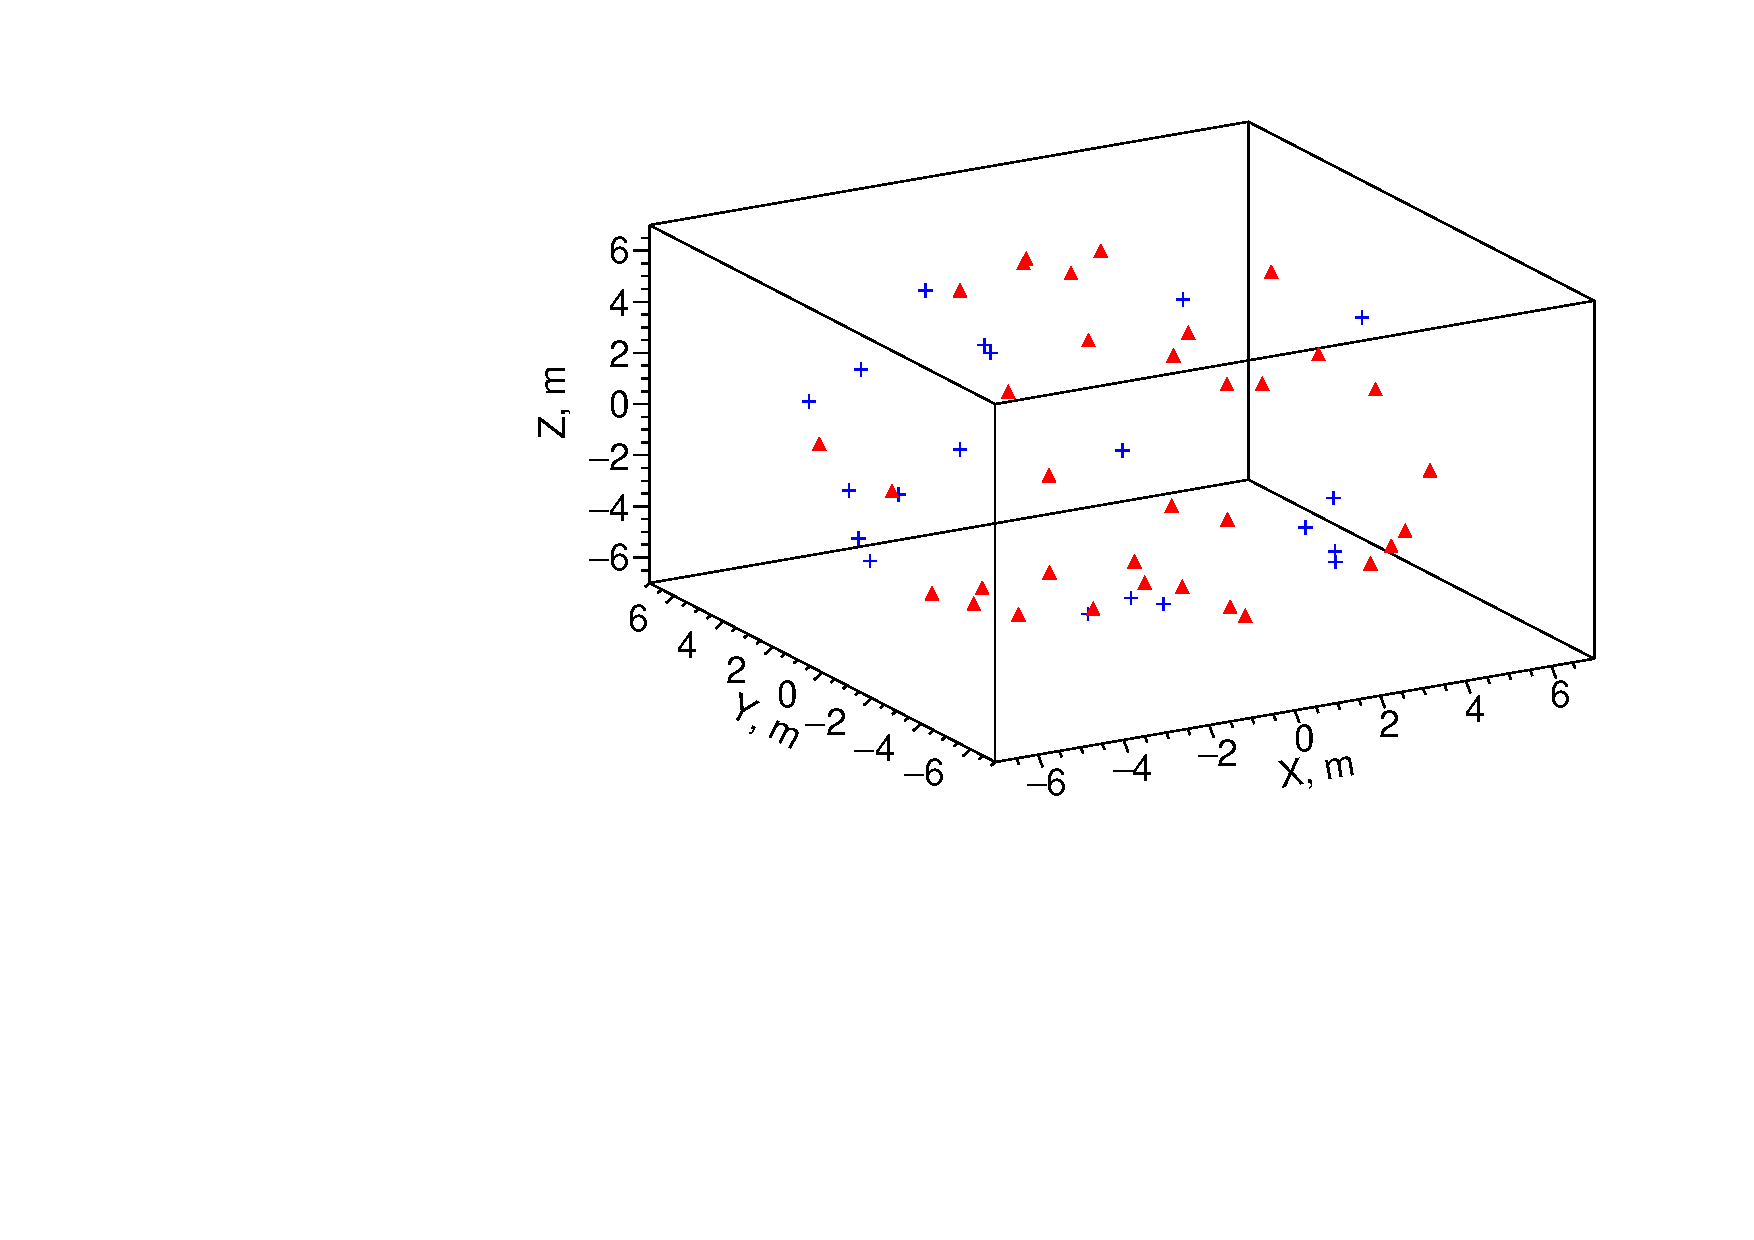
\includegraphics[width=0.45\textwidth]{hDisplay_Te130_evt124_e1257_e1270_cos-0908}
  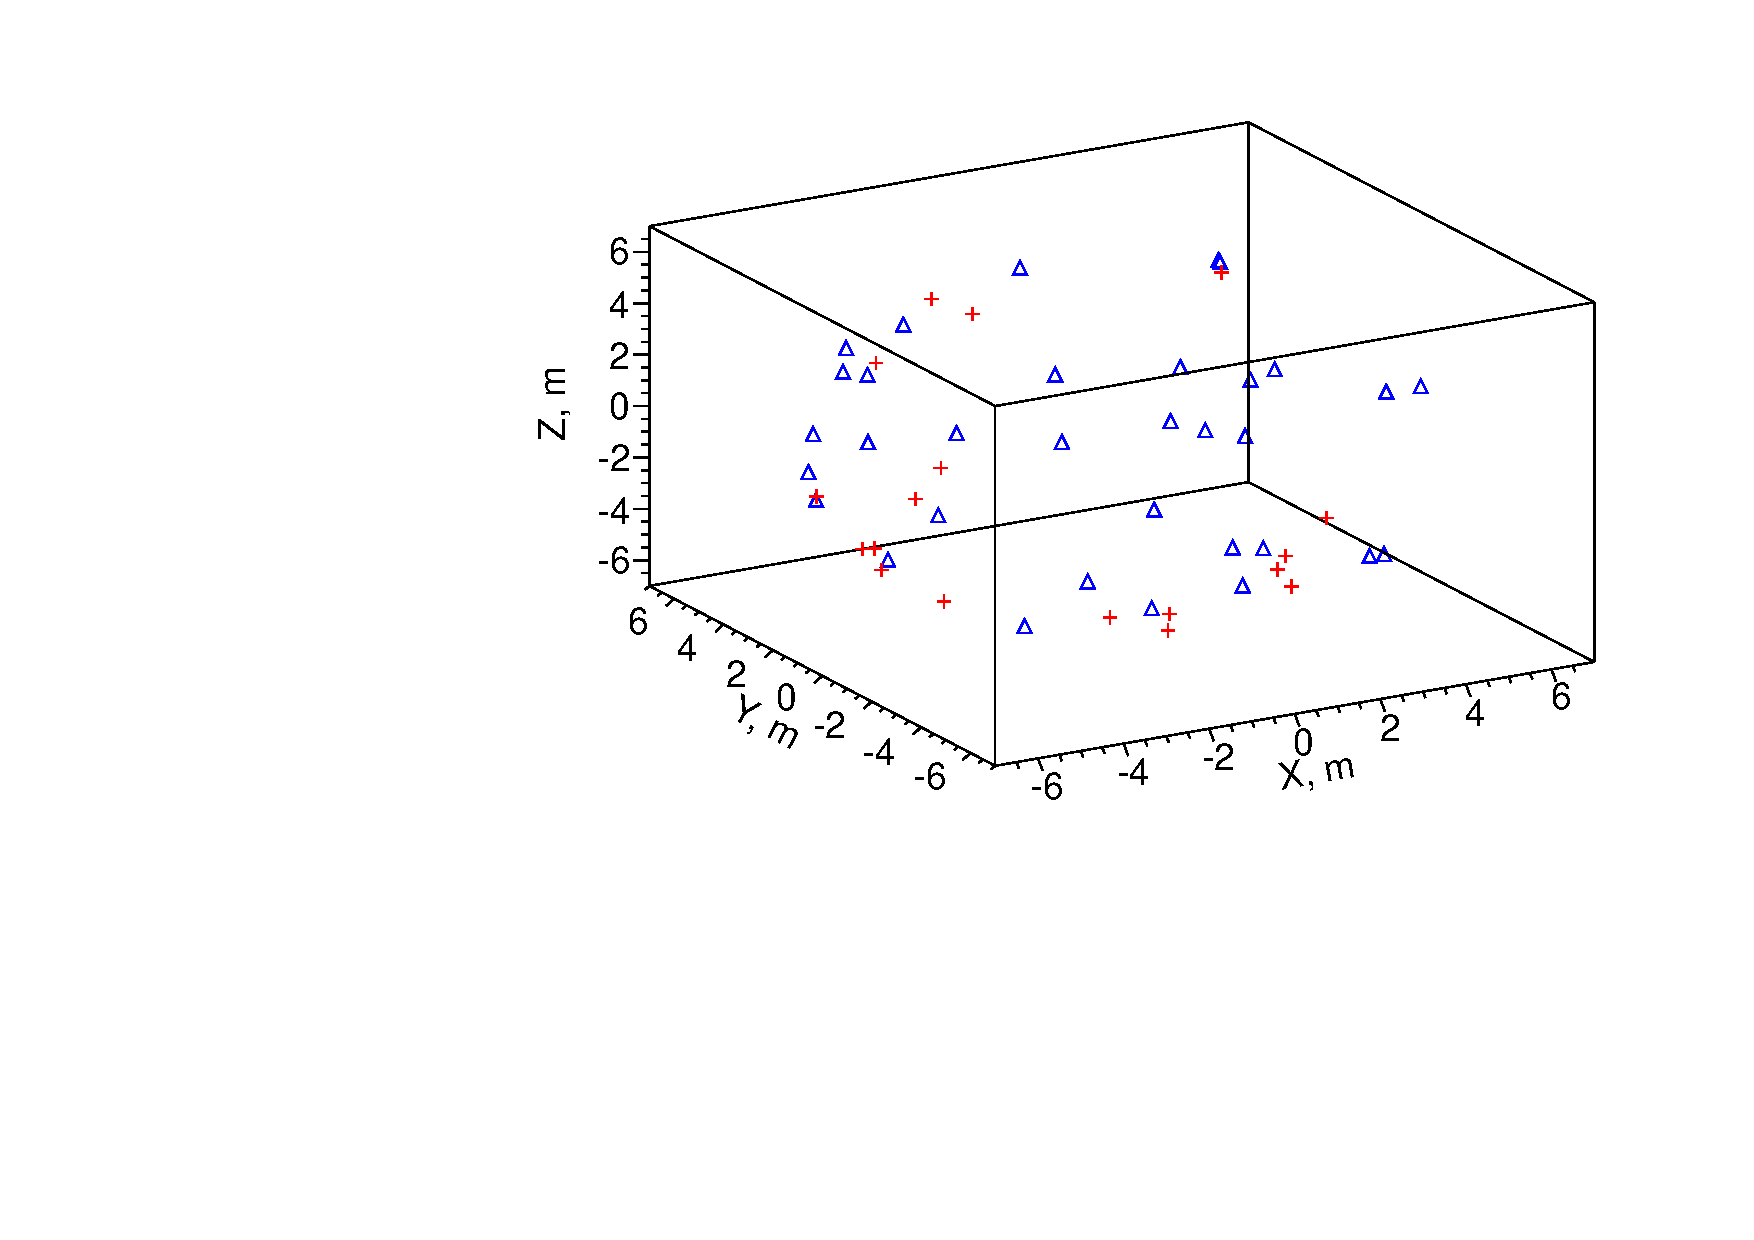
\includegraphics[width=0.45\textwidth]{hDisplay_Te130_evt131_e1264_e1263_cos-0029}
  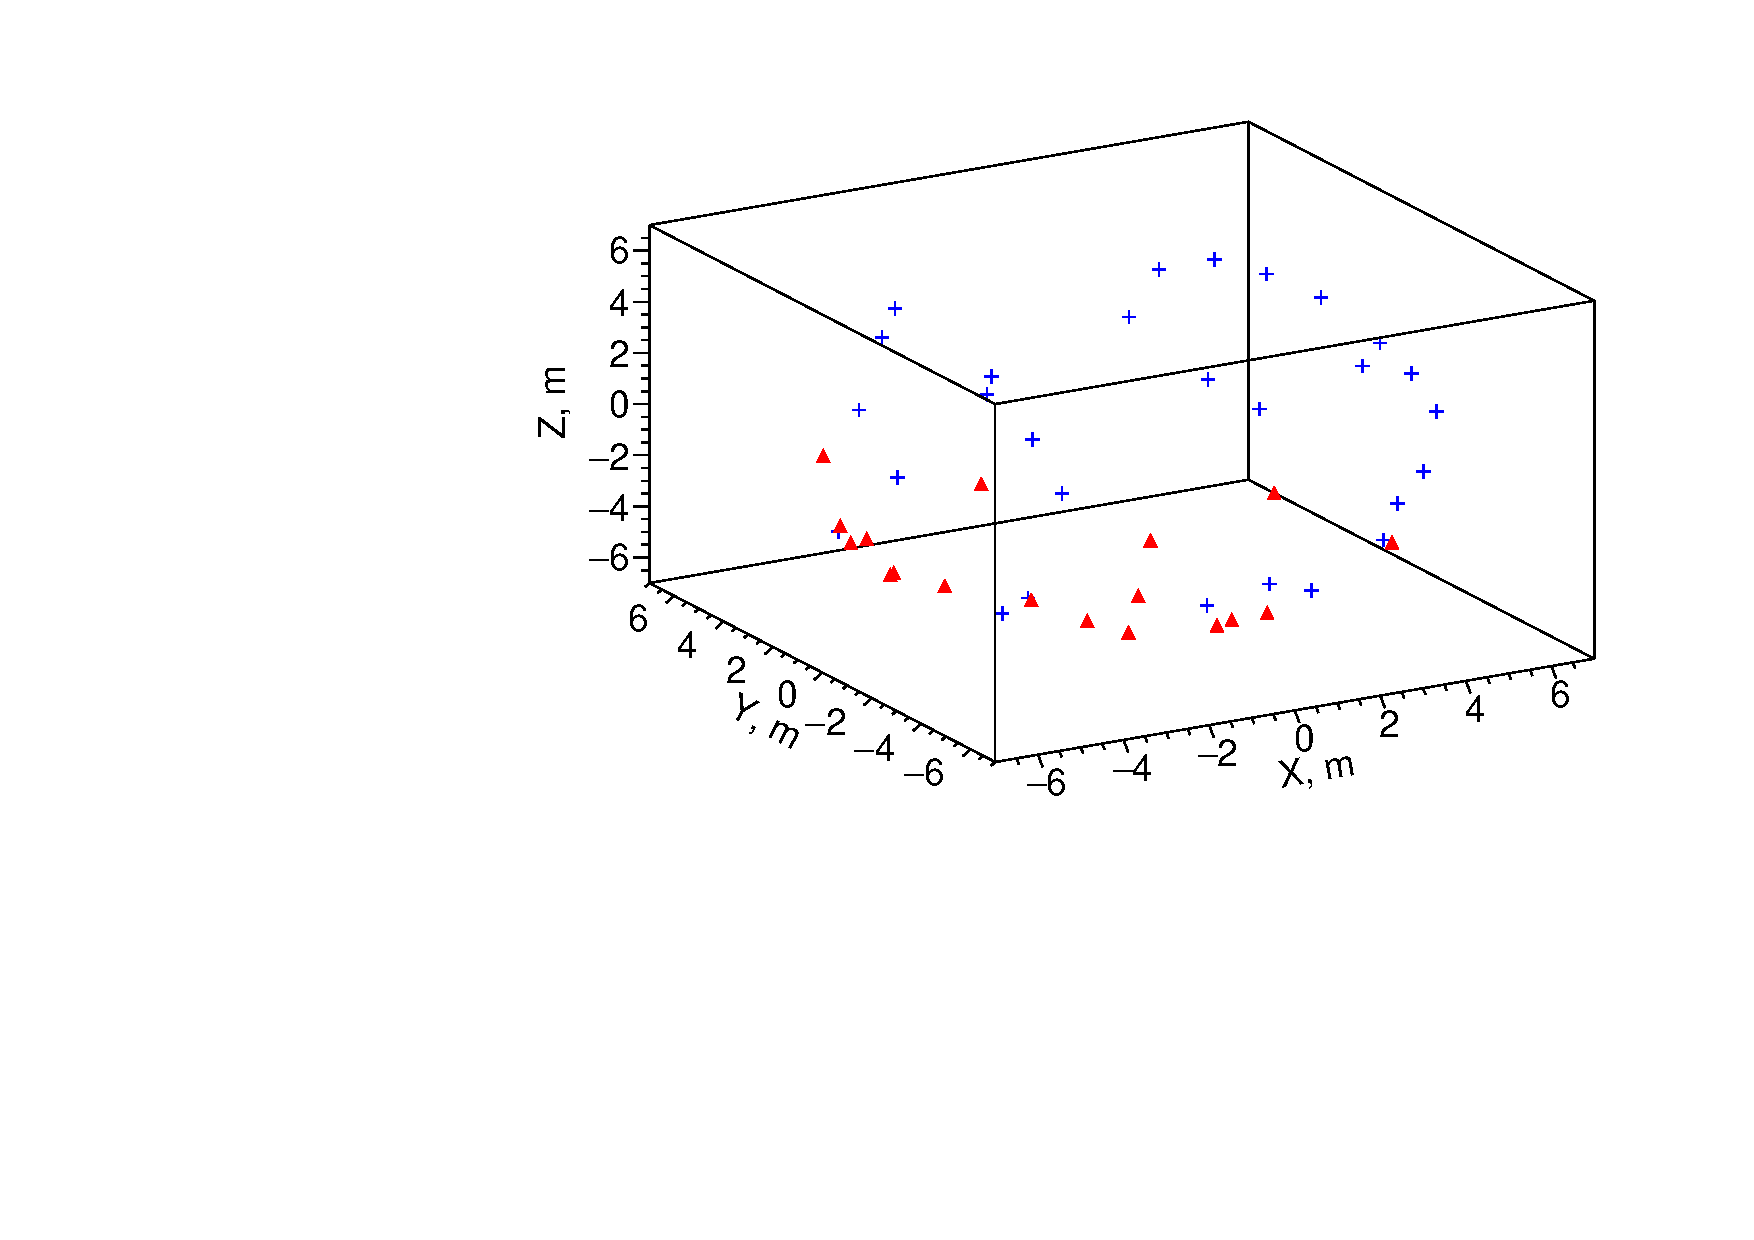
\includegraphics[width=0.45\textwidth]{hDisplay_Te130_evt352_e1186_e1340_cos0888}
  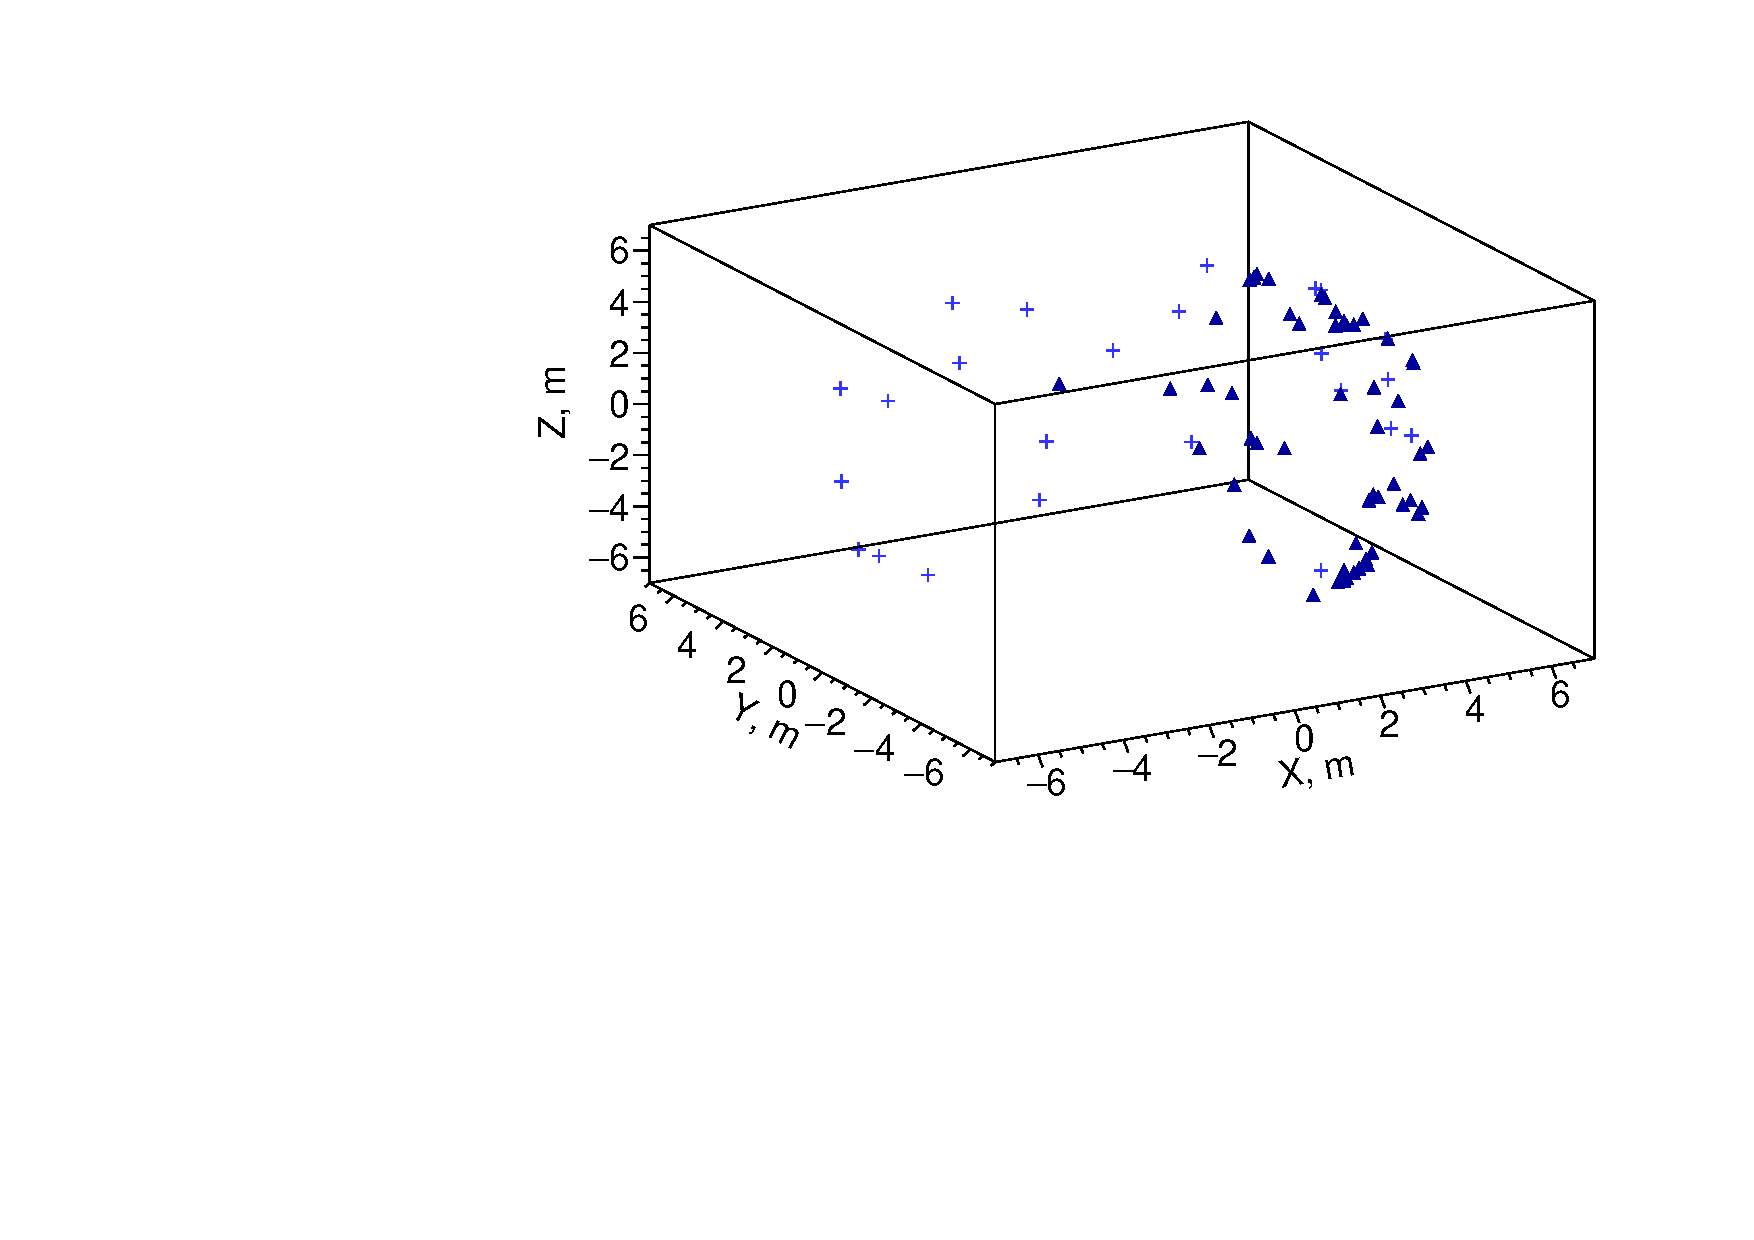
\includegraphics[width=0.45\textwidth]{hDisplay_1el_2p529MeV_33p5ns}
  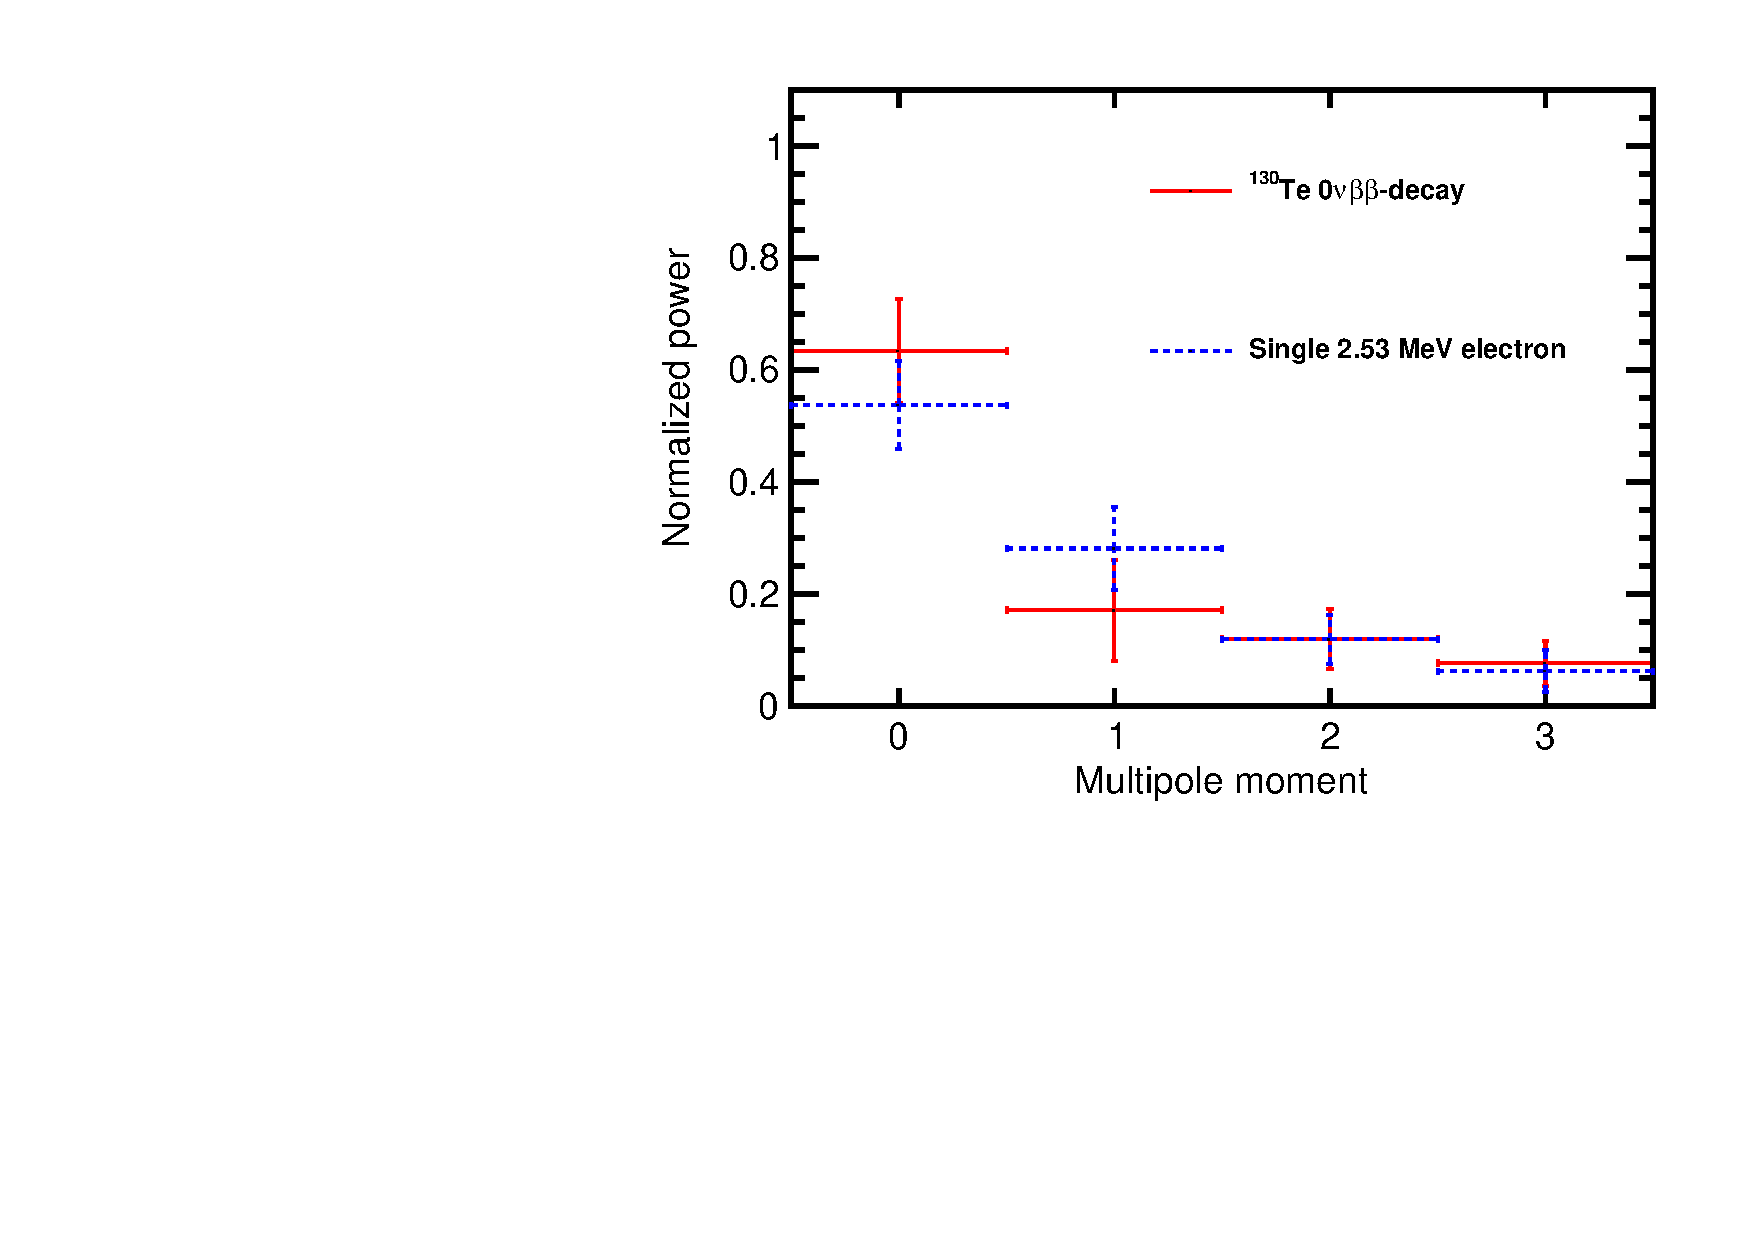
\includegraphics[width=0.8\textwidth]{hMultipleMomentSignal_allLight_VtxSmear0cm_VtxShiftX0cm_33p5ns_center.pdf} 
  \caption{ (\emph{Top and middle rows:} Event display examples for {\Te} 0{\nbb}-decay signal and {\B} background events.
    The default QE and the time cut of 33.5~ns are now applied to cherenkov (\emph{triangles} and scintillation (\emph{crosses}) 
    photons. For the {\Te} 0{\nbb}-decay signal three representative events are shown each closely matching on of the three
    topologies. A typical single electron event is shown for the {\B} background.
    \emph{Top left:} $^{130}$Te 0{\nbb}-decay back-to-back electrons: $E_1$=1.257~MeV, $E_2$=1.270~MeV, 
    cos($\theta$)=-0.908. \emph{Top right:} $^{130}$Te 0{\nbb}-decay electrons at $\sim$90$^{\circ}$: $E_1$=1.264~MeV, $E_2$=1.263~MeV,
    cos($\theta$)=-0.029. \emph{Middle left:} $^{130}$Te 0{\nbb}-decay electrons at $\sim$0$^{\circ}$: $E_1$=1.186~MeV, $E_2$=1.340~MeV,
    cos($\theta$)=0.888. \emph{Middle right:} 2.529~MeV single electron. In all events electrons originate at the center of the detector.
    \emph{Bottom pannel:} Normalized power spectrum $S_l$ calculated for distribution of all PE after the 33.5~ns time cut. 
    {\Te} 0{\nbb}-decay signal (\emph{solid red line}) and {\B} background (\emph{dashed blue line}) topologies are compared.}
\label{fig:Te130_Display}
\end{figure*}


As shown in the middle row of Fig.~\ref{fig:Te130_Display}, 0\nbb~events become indistinguishable from single-track events when the 
angle between the two electrons is small and two Cherenkov clusters overlap. Event topologies of 0\nbb~and \B~events are also 
very similar when only one electron from 0\nbb~ is above the Cherenkov threshold. Therefore spherical harmonics analysis is most 
efficient for events with large angular separation between the two electrons and when both electrons are above Cherenkov threshold.

Being able to distinguish between two-tracks and single-track events using the spherical analyses can allow further cuts to be made.  For example, one might use absolute directional information to suppress single track events where the direction of the track is consistent with the location of a known background such as the sun. Once a single track topology is established, one can use a centroid method (see Ref.~\cite{Directionality}) to reconstruct directionality of the track (or two degenerate tracks) in order to suppress events that are aligned with the direction of \B~solar neutrinos.


\subsection{Spherical Harmonics Analysis and Off-center Events}

In general, the power spectrum $S_l$ is rotation invariant for a given topology only if events originate in the center of the
detector. In order to compare spherical harmonics for events with vertices away from the center a coordinate transformation for each photon 
hit is needed. The necessary transformation applied for each PE within an event is illustrated in Fig.~\ref{fig:SphH_transform}. 
The solid circle in Fig.~\ref{fig:SphH_transform}~has a radius R and shows the actual detector boundaries. The dotted circle shows a new 
sphere with the same radius R, which now has the event vertex in its center. The radius vector of each PE is stretched or shorten to 
its intersection with this new sphere using the transformation, $\vec{r}^{,}_{PE} = \frac{\vec{a}}{|\vec{a}|} \cdot R$, 
where $\vec{r}^{,}_{PE}$ is a new radius vector of a PE and $\vec{a}=\vec{r}_{PE} - \vec{r}_{vtx}$ with $\vec{r}_{PE}$ and $\vec{r}_{vtx}$ 
being radius vectors of the PE and the vertex in the original coordinates, respectively.

\begin{figure*}[h]
  \centering
%  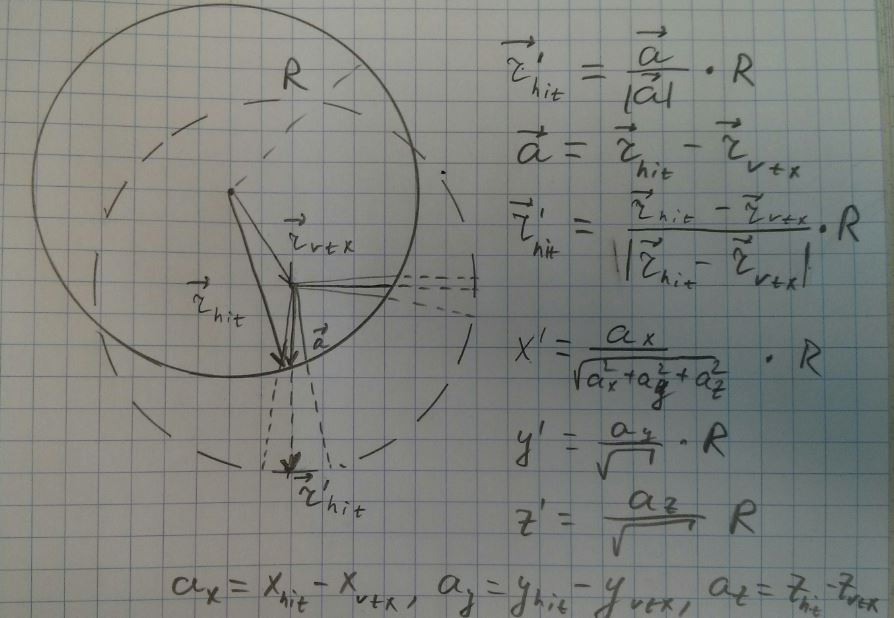
\includegraphics[width=0.95\textwidth]{SphH_transform_sketch.JPG}
  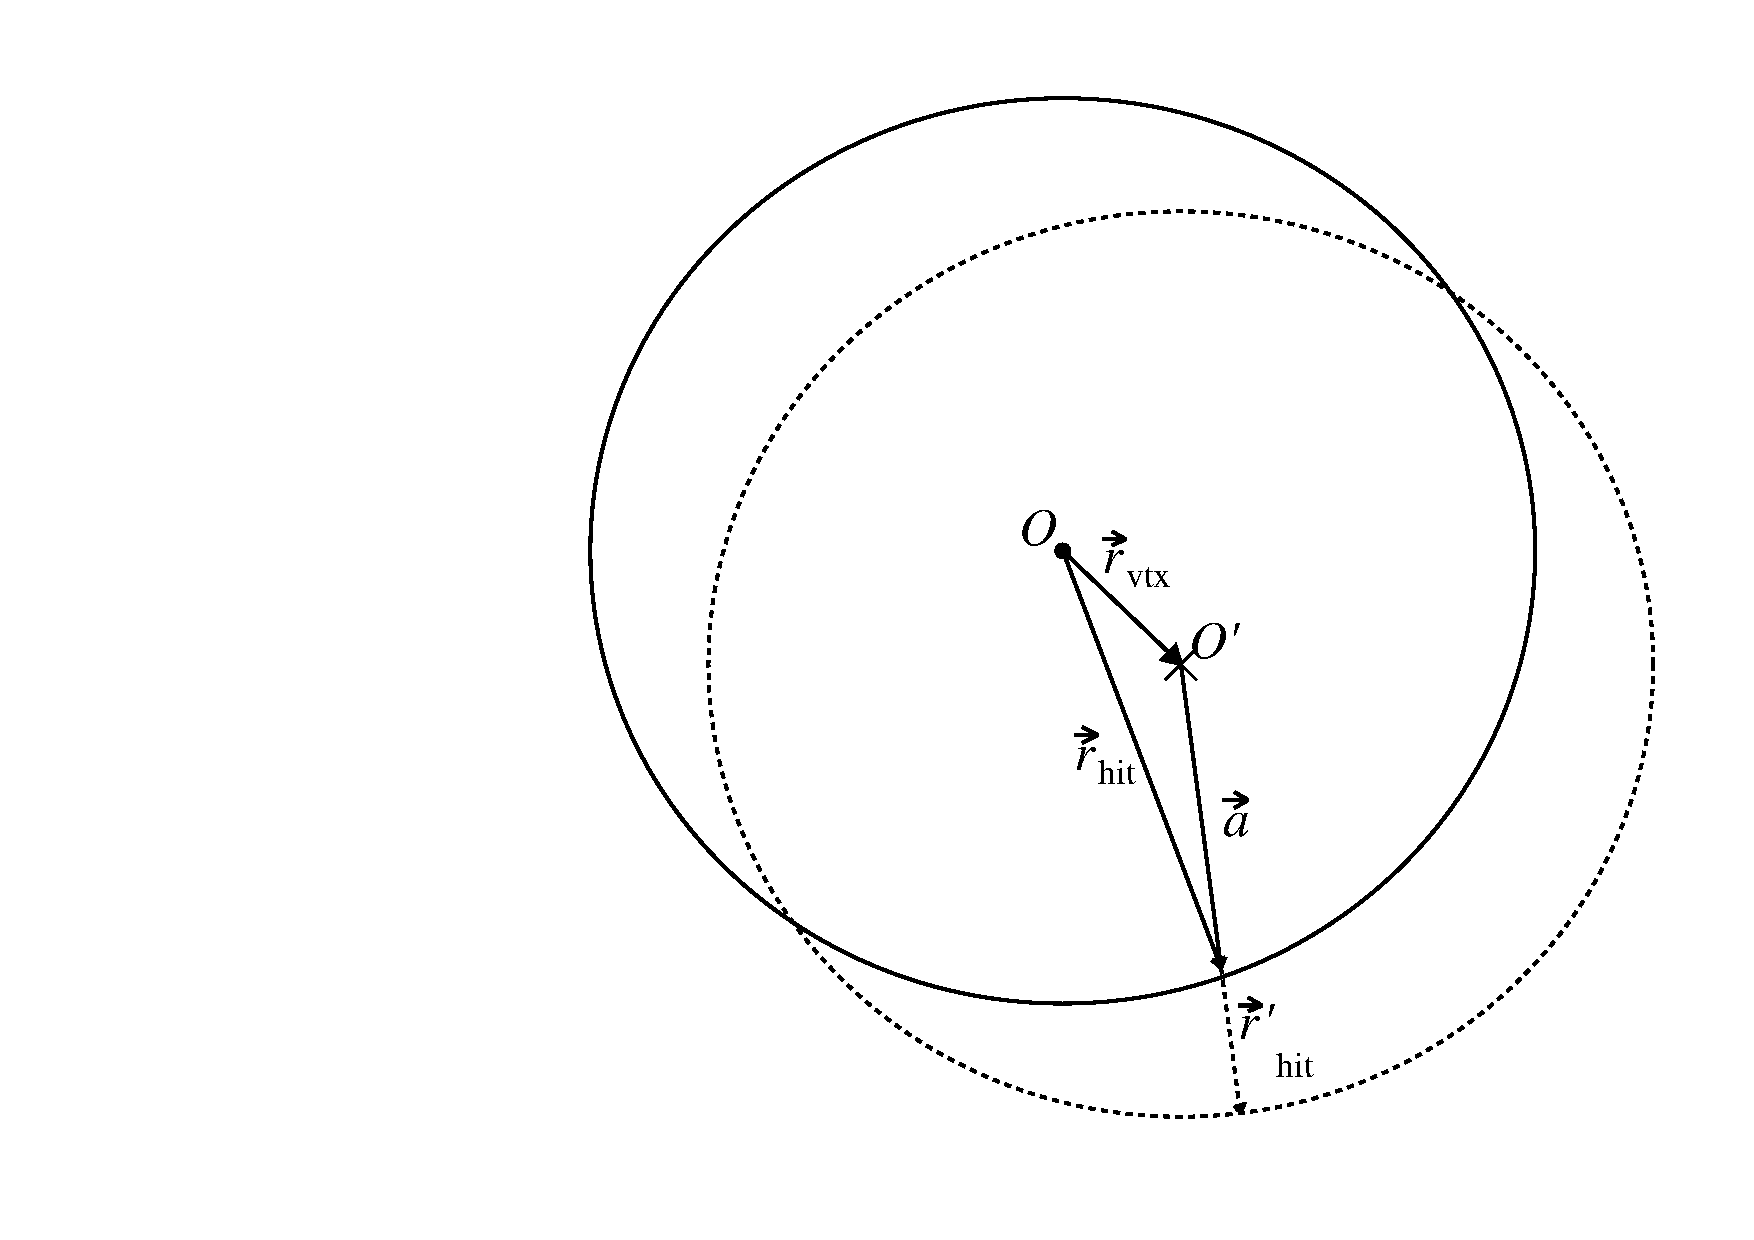
\includegraphics[width=0.8\textwidth]{SphH_transform.pdf}
  \caption{Coordinate transformation applied to events that are
    off-center. Solid circle schematically shows actual detector
    boundaries. Dotted circle shows a new sphere of radius R$=$6.5~m
    with the event vertex position in the center. The radius vector of
    each photon hit is stretched or shorten until intersection with
    this new sphere using transformation $\vec{r}^{,}_{hit} =
    \frac{\vec{a}}{|\vec{a}|} \cdot R$. Where $\vec{r}^{,}_{hit}$ is a
    new radius vector of the photon hit, $R$ is detector sphere radius,
    and $\vec{a}=\vec{r}_{hit} - \vec{r}_{vtx}$ with $\vec{r}_{hit}$
    and $\vec{r}_{vtx}$ being radius vectors of the photon hit and
    vertex position in original coordinates and correspondingly.}
  \label{fig:SphH_transform}
\end{figure*}


\subsection{Implementation of the spherical harmonics analysis}

Numerical calculation of the power spectrum is implemented as follows.
For each event, we create a 2-D histogram, $\theta$ vs $\phi$, with the distribution of PEs on the detector surface. We then treat this 
histogram as a function $f(\theta,\phi)$ where the value of the function for any pair of $\theta$ and $\phi$ is equal to the number of 
PE in the histogram bin corresponding to that pair.

Coefficients $f_{lm}$ from Eq.~\ref{eq3} are calculated using a Monte Carlo integration technique. Variables $S_l$'s are calculated using 
Eqs.\ref{eq4} - \ref{eq6}. {\bf Also need to provide reference to the libraries for Legandre polinomials.}

%----------LARGE COMMENT BLOCK BEGINS-------------
\begin{comment}

\textbf{ I'm thinking of removing Figs~\ref{fig:SL_topologies_CHE}-\ref{fig:SL_topologies_all}, thus the following paragraphs are in Italic. 
I think bottom pannels in Figs.~\ref{fig:ThreeTopologies_Display_5MeV}-\ref{fig:Te130_Display} convey enough info that it only make sense to use
$S_0$ and $S_1$}

\begingroup
  \itshape
To illustrate spherical harmonics analysis technique we compare distributions of $S_0$, $S_1$, $S_2$, and $S_3$ for the three representative event topologies described in Sec.~\ref{subsec:topology}. Almost all the information about event topology is carried by Cherenkov light. Therefore we first show spherical harmonics for back-to-back,  90$^{\circ}$ and single track topologies based on Cherenkov PEs only (see Fig.~\ref{fig:SL_topologies_CHE}).

Two top panels of Fig.~\ref{fig:SL_topologies_CHE} show 2-dimensional distributions, S0 vs S1 and S2 vs S3, to demonstrate that all four $S_l$'s provide separation between event topologies. No QE is applied in simulation of these events. We also introduce a 1-dimensional variable, S01 (bottom panel of Fig.~\ref{fig:SL_topologies_CHE}), that has the best separation power for majority of event topologies considered in this paper. $S_{01}$ is defined as a projection of S$_1$ vs S$_2$ distribution onto a linear fit of this 2-D distribution.

%\endgroup

\begin{figure*}[h]
  \centering
  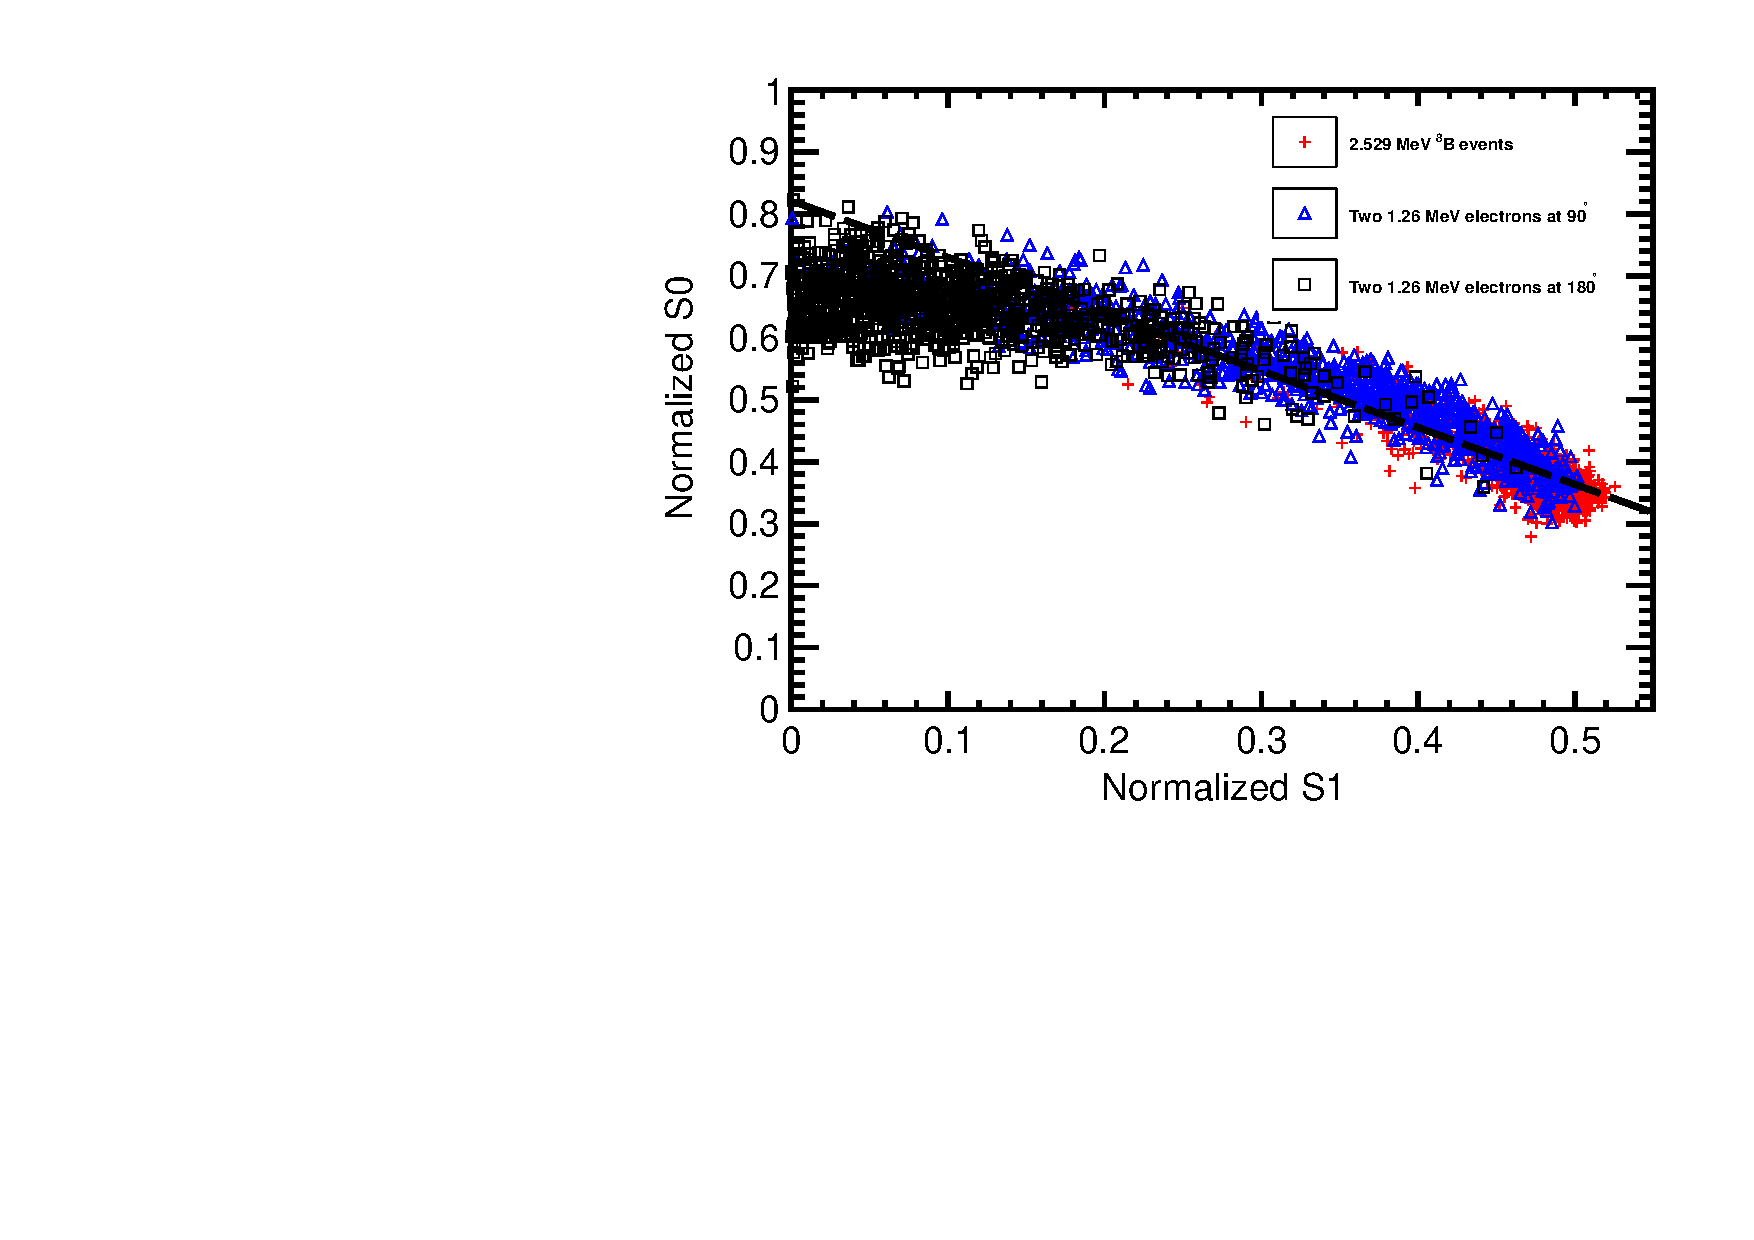
\includegraphics[width=0.49\textwidth]{ALL/hS0vsS1_topologies_CHELight_VtxSmear0cm_VtxShiftX0cm_33p5ns_center.pdf}
  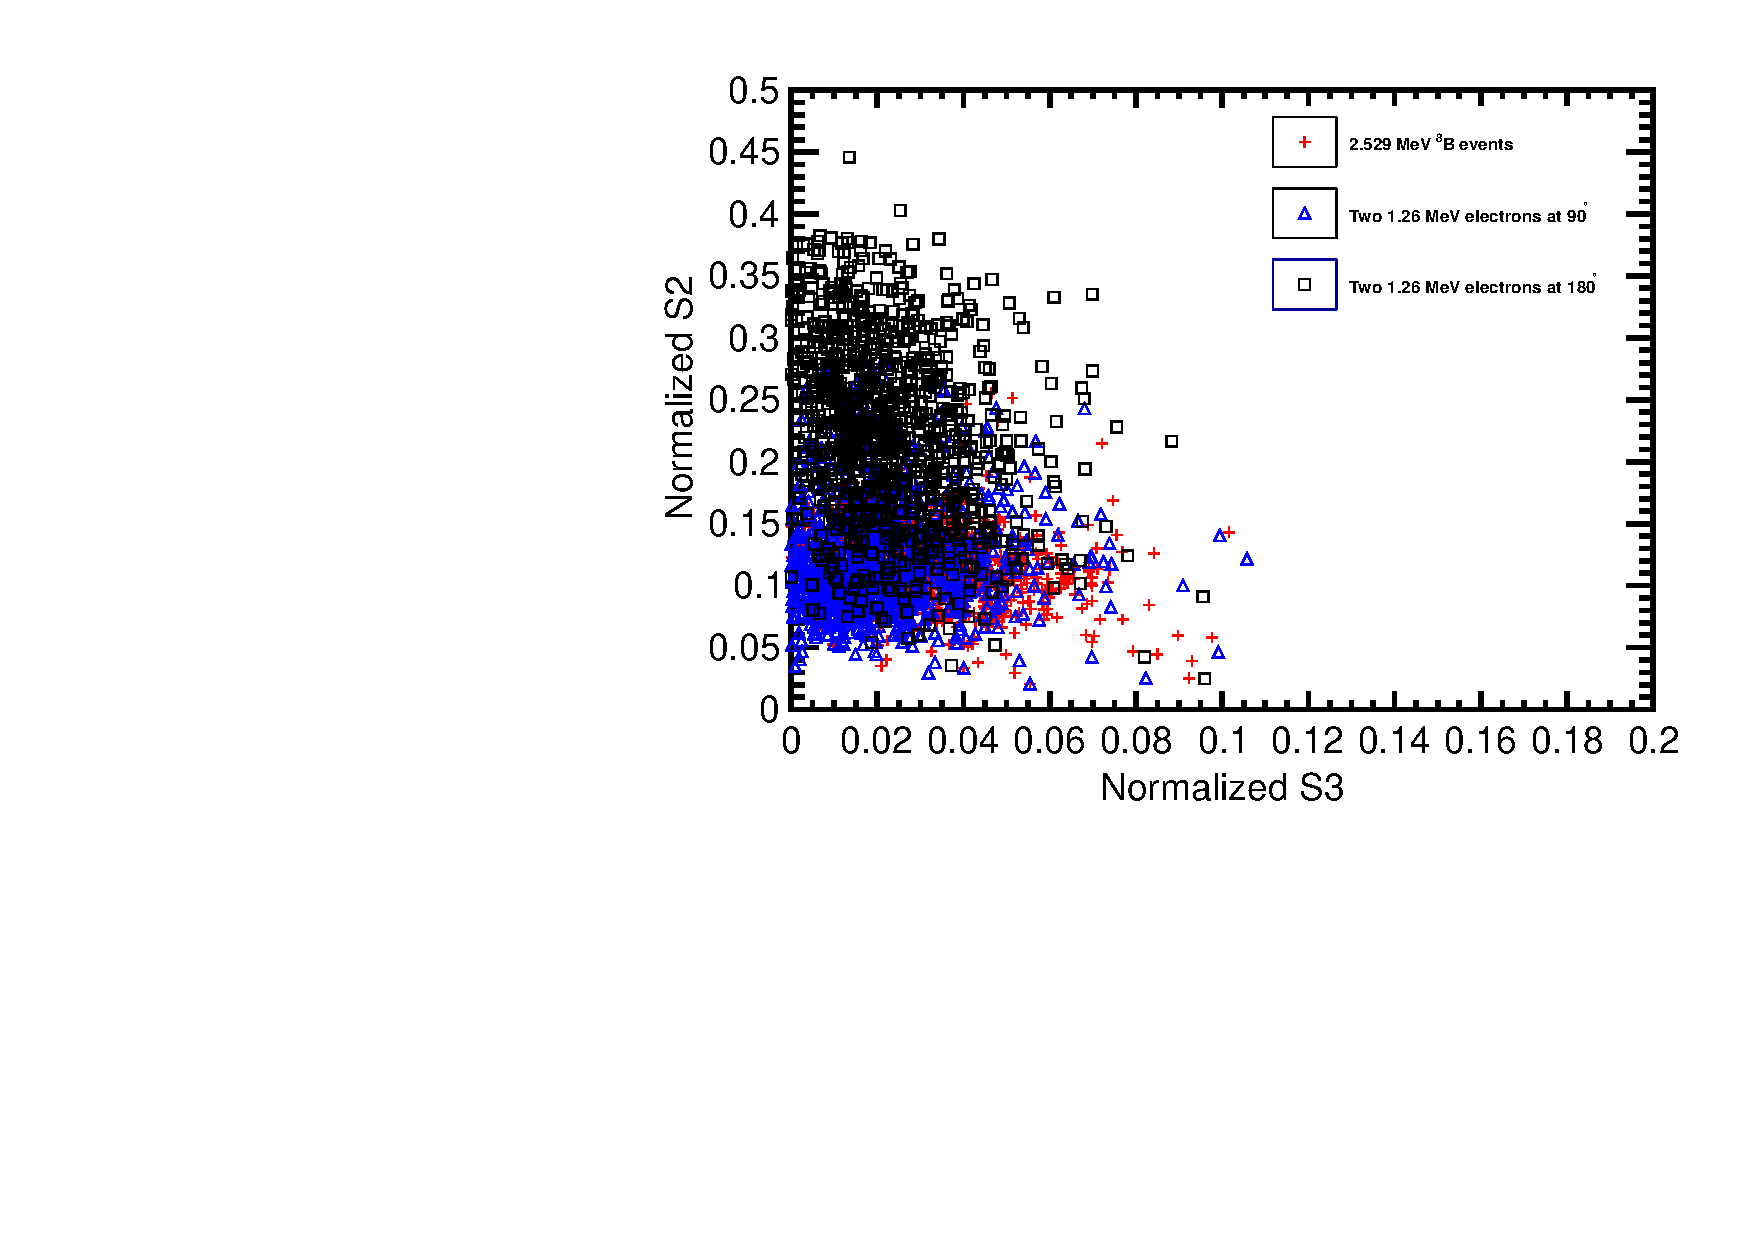
\includegraphics[width=0.49\textwidth]{ALL/hS2vsS3_topologies_CHELight_VtxSmear0cm_VtxShiftX0cm_33p5ns_center.pdf}
  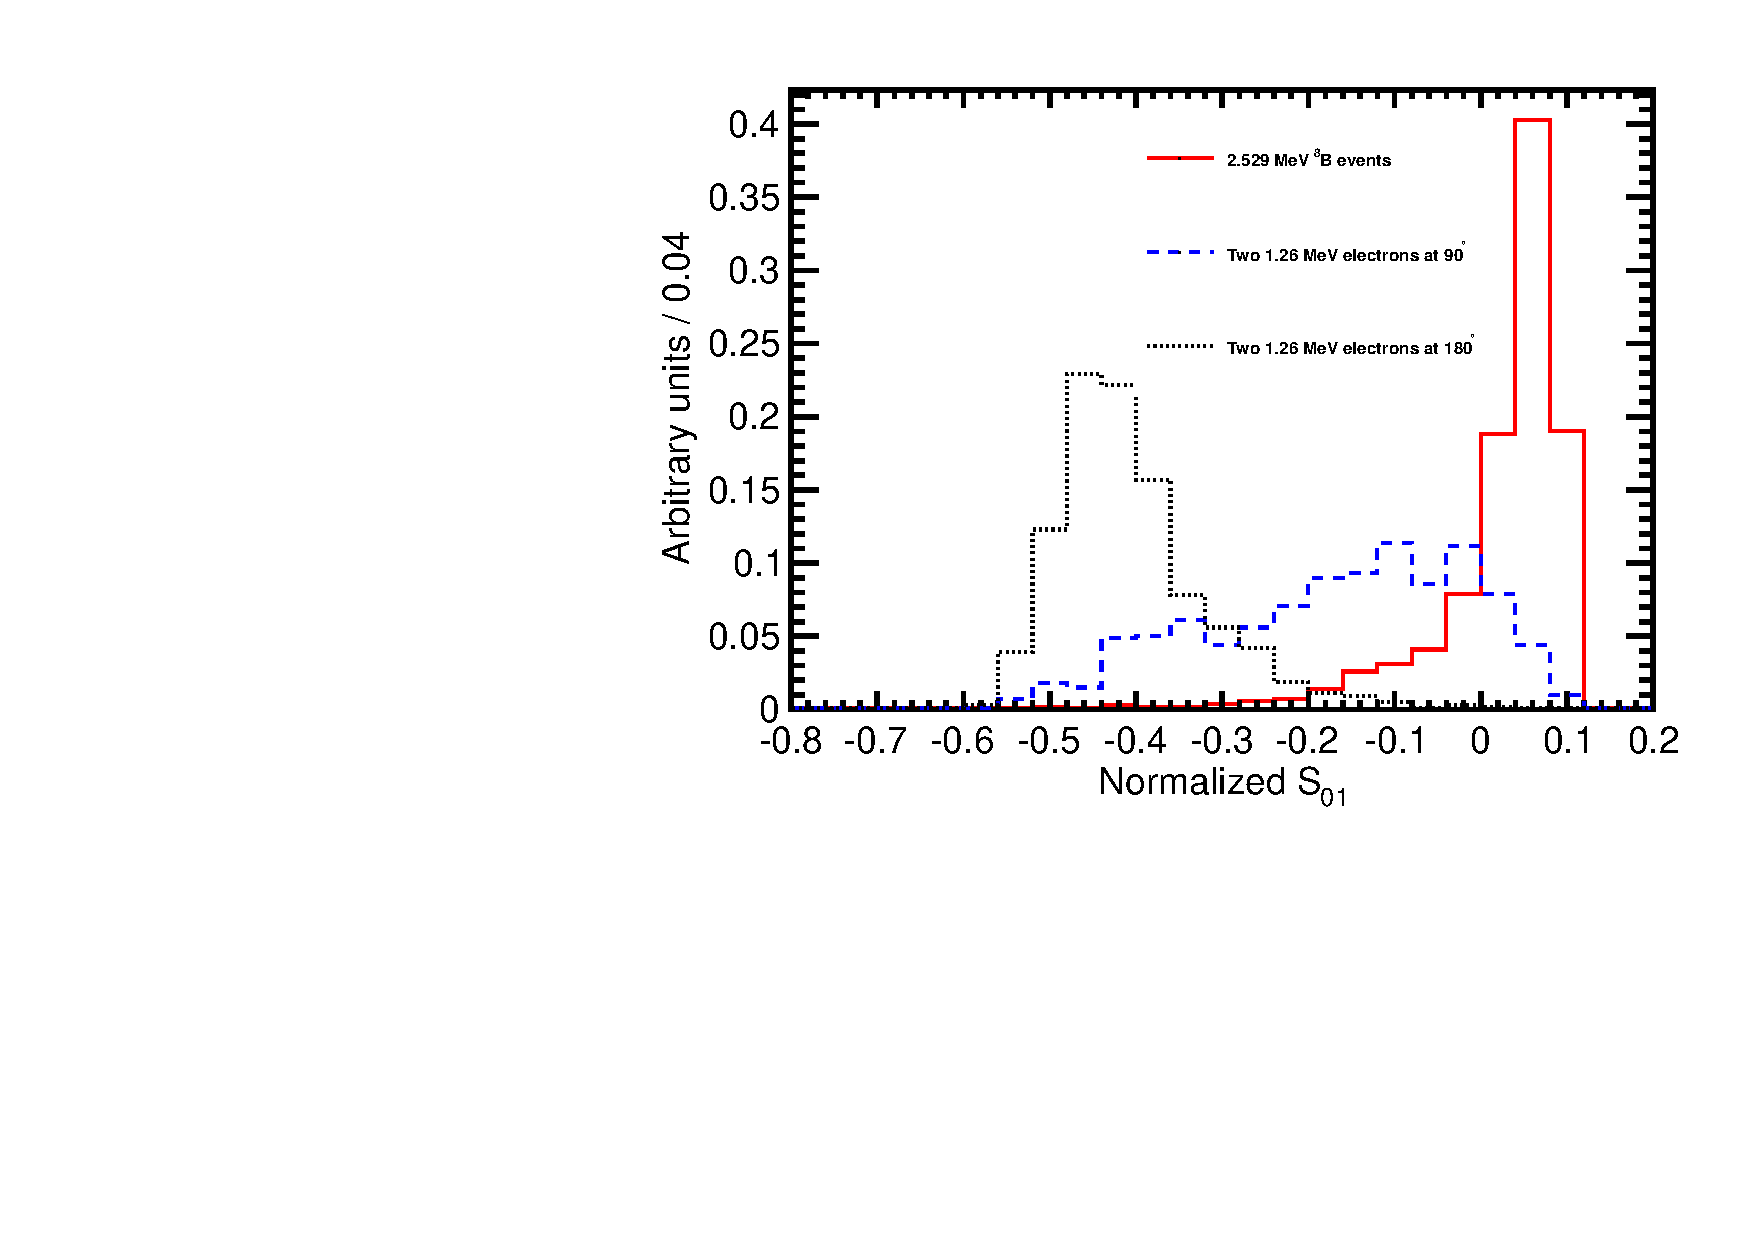
\includegraphics[width=0.9\textwidth]{ALL/hS01_topologies_CHELight_VtxSmear0cm_VtxShiftX0cm_33p5ns_center.pdf}
  \caption{Spherical harmonics for three event topologies: two
    back-to-back 1.26~MeV electrons (\emph{black squares and black
      dotted line}), two 1.26~MeV electrons at 90$^{\circ}$ angle
    (\emph{blue triangles and blue dashed line}), and a single
    2.529~MeV electron representing $^{8}$B background (\emph{red
      crosses and red solid line}). Simulation of 1000 events
    originated at the center of the sphere. Perfect separation between
    Cherenkov and scintillation light is implemented in this
    simulation by using only Cherenkov photons. \emph{Top left:} $S_0$
    versus $S_1$ scatter plot. Black dotted line is a linear fit of
    the 90$^{\circ}$ topology and $^{8}$B events. Variable $S_{01}$ is
    defined as a projection of 2D distribution onto this linear
    fit. \emph{Top right:} $S_2$ versus $S_3$ scatter
    plot. \emph{Bottom:} $S_{01}$ distributions for the three
    topologies. These distributions are normalized to unit area for
    shape comparison.}
  \label{fig:SL_topologies_CHE}
\end{figure*}


The effects due to the presence of scintillation light and applying the default QE are shown in Fig.~\ref{fig:SL_topologies_all}. Spherical harmonics of the same three representative event topologies are now calculated using early light (photons with arrival time less than 33.5~ns) that contains both directional Cherenkov light and uniform scintillation light. The of number PE seen by each tube is reduced by the default QE. In this more realistic scenario, the higher order multiple moments, S2 and S3, no longer provide noticeable separation between different event topologies.


\begin{figure*}[h]
  \centering
  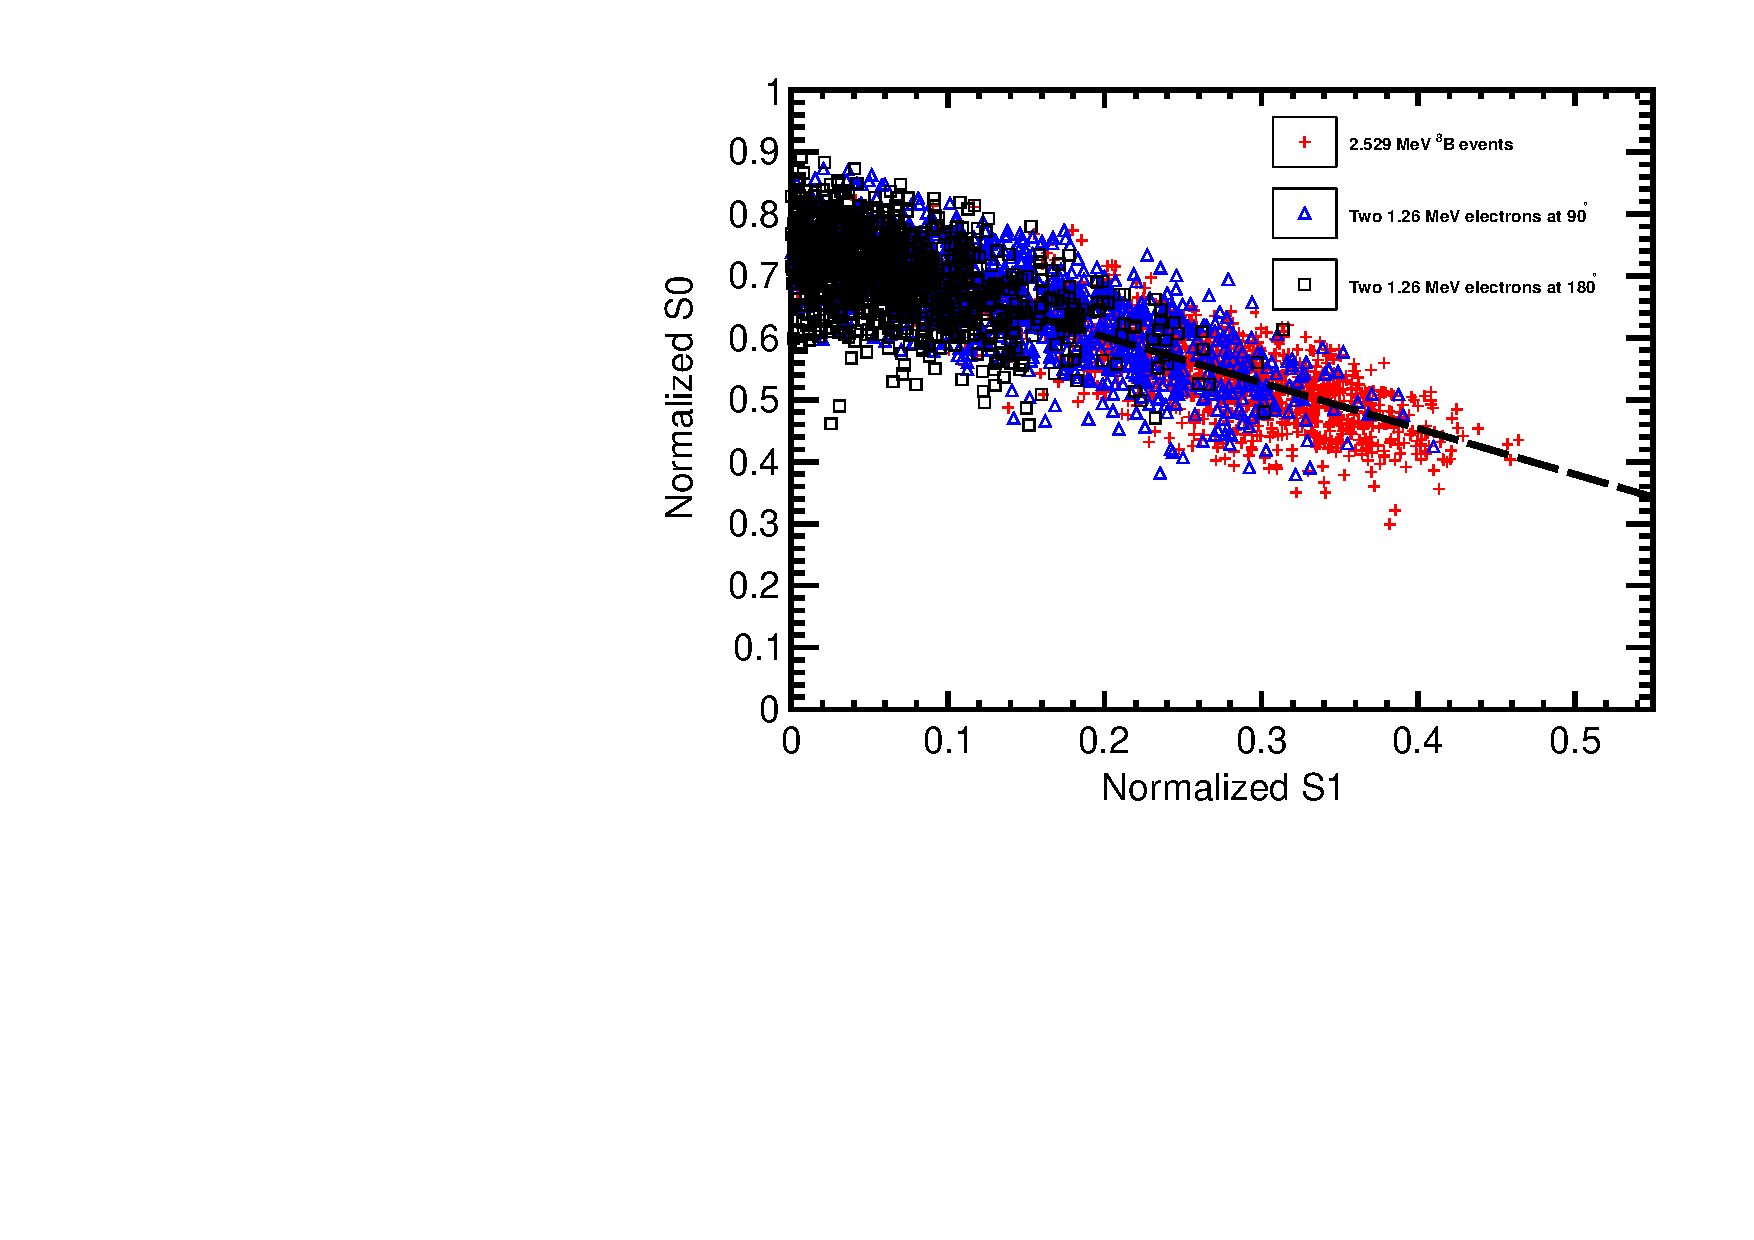
\includegraphics[width=0.49\textwidth]{hS0vsS1_topologies_allLight_VtxSmear0cm_VtxShiftX0cm_33p5ns_center.pdf}
  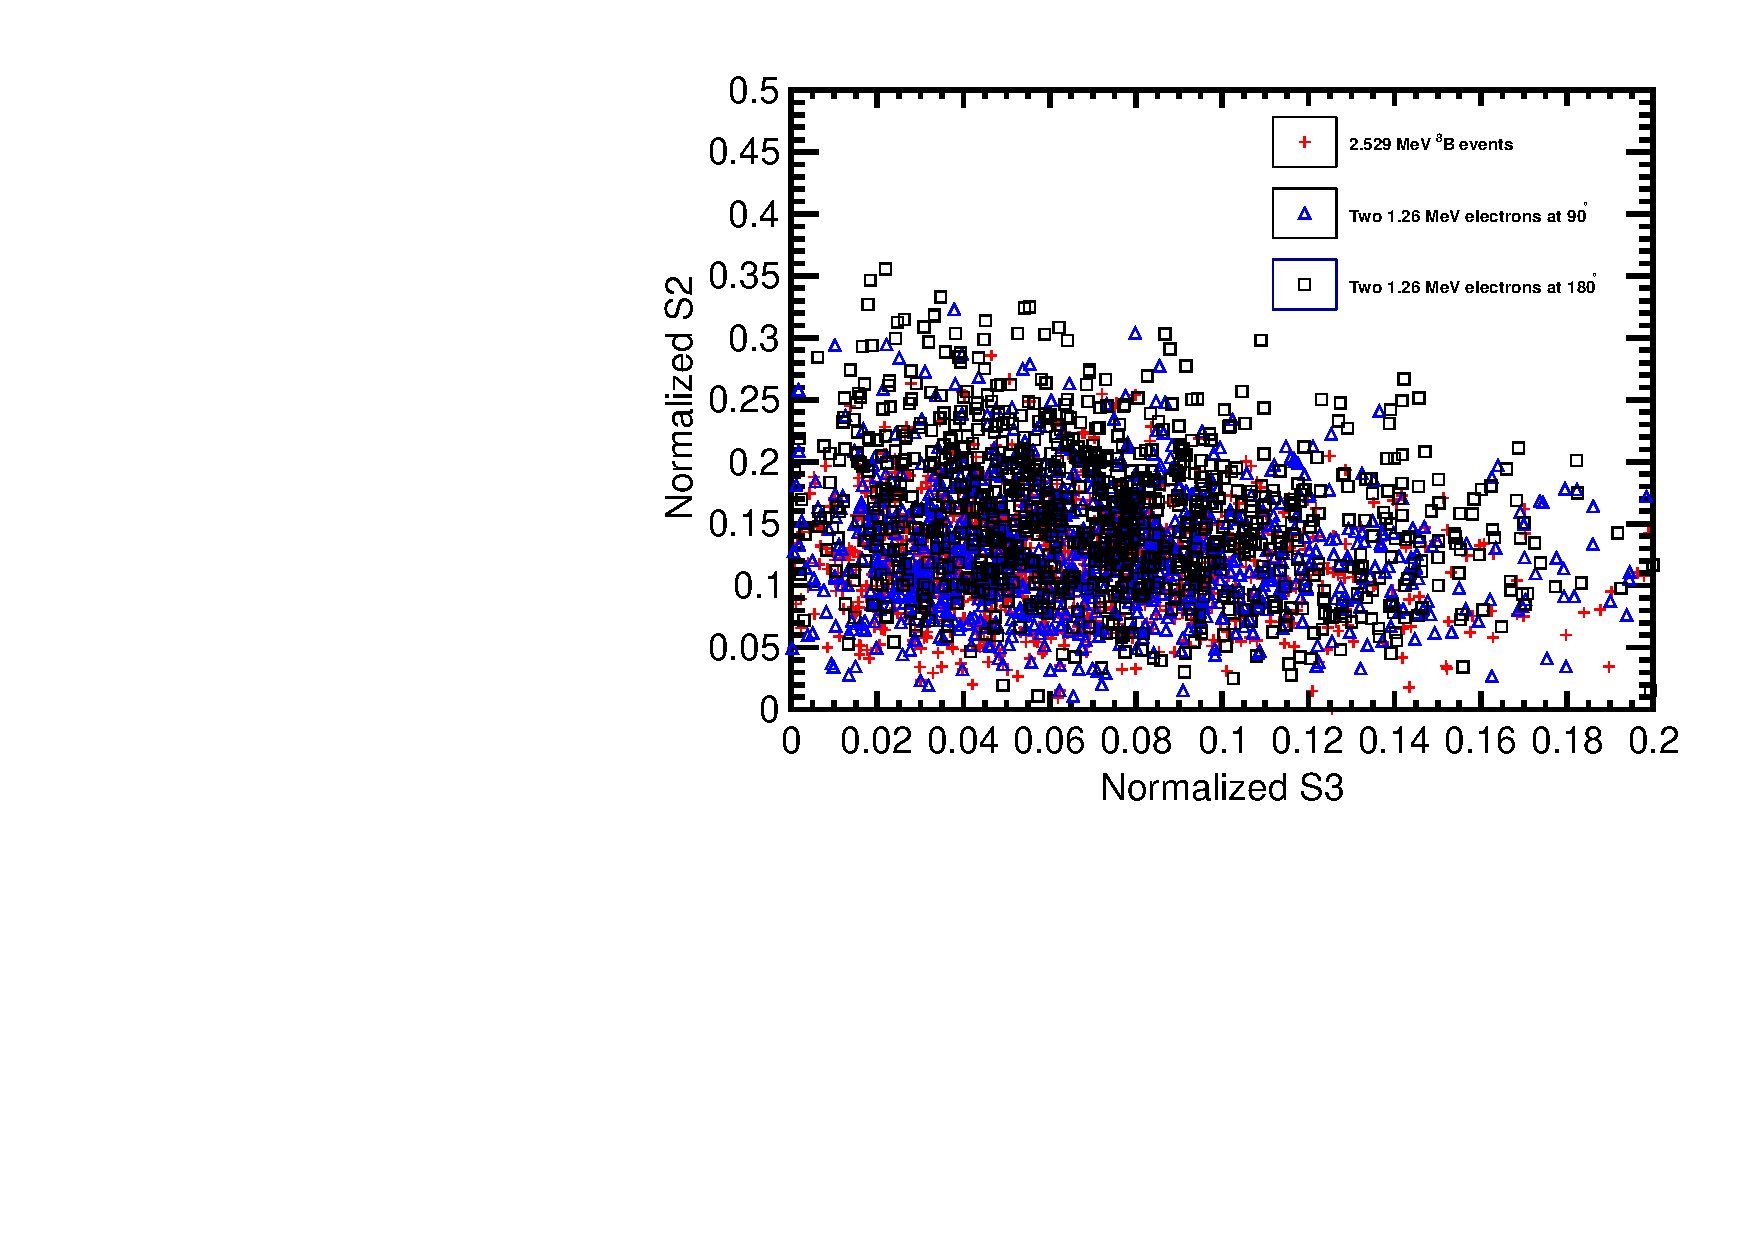
\includegraphics[width=0.49\textwidth]{hS2vsS3_topologies_allLight_VtxSmear0cm_VtxShiftX0cm_33p5ns_center.pdf}
  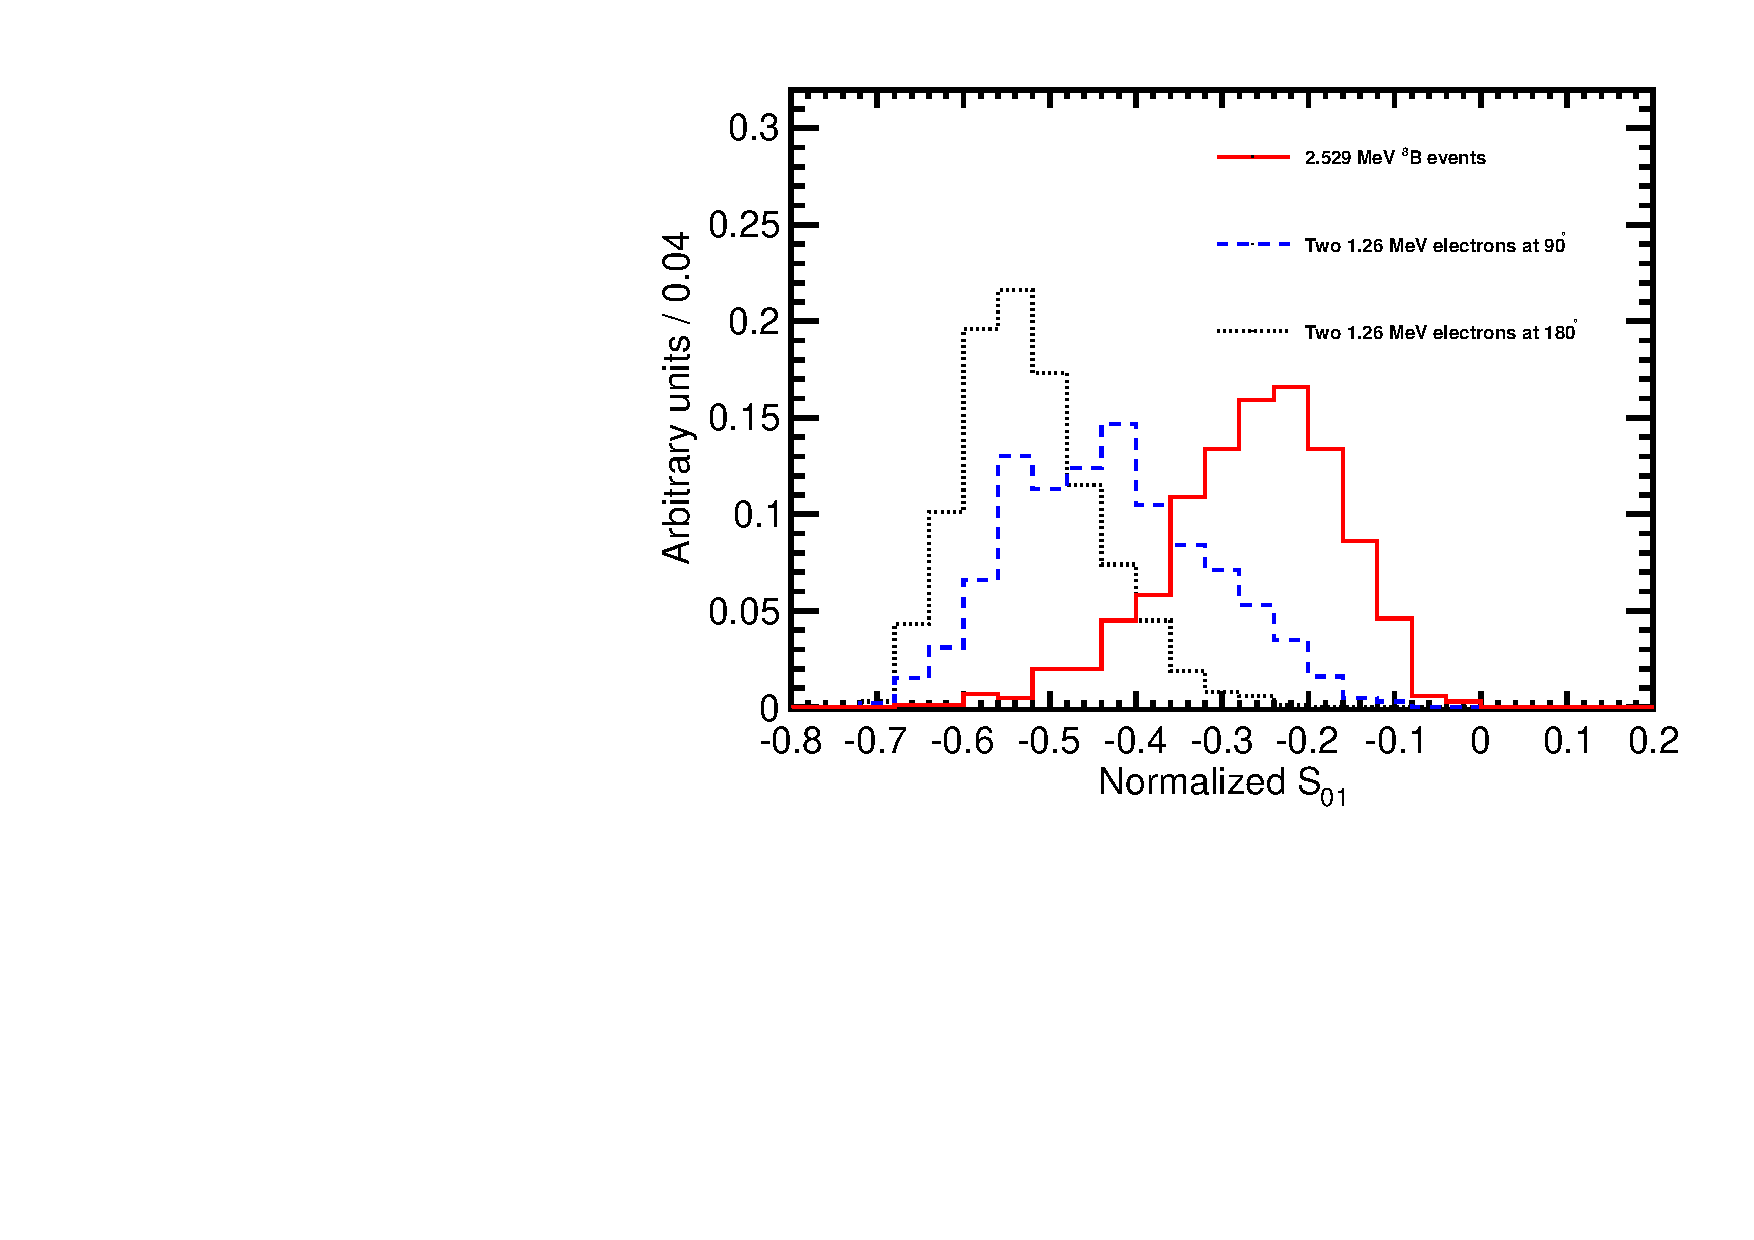
\includegraphics[width=0.9\textwidth]{hS01_topologies_allLight_VtxSmear0cm_VtxShiftX0cm_33p5ns_center.pdf}
  \caption{Spherical harmonics for three event topologies: two
    back-to-back 1.26~MeV electrons (\emph{black squares and black
      dotted line}), two 1.26~MeV electrons at 90$^{\circ}$ angle
    (\emph{blue triangles and blue dashed line}), and a single
    2.529~MeV electron representing $^{8}$B background (\emph{red
      crosses and red solid line}). Simulation of 1000 events
    originated at the center of the sphere. Separation between
    Cherenkov and scintillation light is implemented 33.5~ns cut on
    the photon arrival time. Perfect vertex reconstruction - true
    vertex position is used. \emph{Top left:} $S_0$ versus $S_1$
    scatter plot. Black dotted line is a linear fit of the
    90$^{\circ}$ topology and $^{8}$B events. Variable $S_{01}$ is
    defined as a projection of 2D distribution onto this linear
    fit. \emph{Top right:} $S_2$ versus $S_3$ scatter
    plot. \emph{Bottom:} $S_{01}$ distributions for the three
    topologies. These distributions are normalized to unit area for
    shape comparison}
\label{fig:SL_topologies_all}
\end{figure*}


\endgroup
\end{comment}
%----------LARGE COMMENT BLOCK ENDS-------------


\subsection{Spherical harmonics analysis of \C~background events}
\label{subsec:c10_spherical_harmonics}
\textbf{This subsection needs more details and a plot showing 0\nbb/\C~separation using sherical harmonics in the default Geant-4 configuration.}
Ortho-positronium formation is not included in the default Geant-4 package. Therefore photon arrival time to the detector surface is not 
properly simulated.
